\chapter{和积、贝特-菊池、期望传播}

本章我们将开始讨论 Message-passing 的变分解释。
首先从 Sum-product 算法,也就是 Belief-ropagation 开始。
如 2.5 小节所述,Sum-product 是一种可用于树结构图的精确算法,可以用分治进行表达。
然而,Sum-product 的 Update 是在局部进行的,完全可以应用到带环图上,这就是 Sum-product 或 Belief-propagation 的“循环(Loopy)”形式。
在存在环的情况下,Sum-product 没有收敛性或正确性的一般证明,但它仍然被广泛用于计算近似 Marginals。
本章的第一部分将在 Bethe 近似的条件下描述和积更新的变分公式。
虽然这种近似最早可以追溯到 Bethe 的工作,但它与 Sum-product 的联系最早是由 Yedidia 等人阐明的。
然后我们描述几类 Bethe 近似的拓展,包括 Kikuchi-clustering 和其他基于超图(Hypergraph)的方法。
最后我们描述 Expectation-propagation 算法和相关的 Moment-matching 方法,这些也是基于 Bethe-like 近似的变分方法。

\section{和积与贝特近似}

Bethe 近似最简单的实例是一个最多只涉及变量对的无向图 $G = (V, E)$,我们把这种模型称为 Pairwise MRF \footnote{
    原则上通过引入适当的辅助变量,任何无向图模型都可以转化成等价的 Pairwise 形式,并且应用 Bethe 近似,具体操作可见附录 E.3。
    直接处理高阶 Interactions 也可以,相应的近似方法见 4.2 小节。
}。Sum-product 在离散随机变量和 Gaussian 随机变量中用的最多,我们主要讨论离散的情况,节点 $s \in V$ 的相关变量 $X_s$ 取值为 $X_s = \{0, 1, \dots, r_{s-1}\}$。

在离散的情况下,一般变分原理 (3.45) 根据所选的充分统计量 $\phi$ 的不同而具有不同的形式。
回顾一下 3.4.1 小节中对正则过完备表示的定义 (3.34),充分统计量选用了事件 $\{X_s = j\}$ 和 $\{X_s = j, X_t = k\}$ 的 Indicator-functions。
在这种条件下,我们把指数族定义为如下形式:
\begin{equation}
    p_{\theta}(x) \propto \exp\{\sum_{s \in V}\theta_s(x_s) + \sum_{(s, t) \in E}\theta_{st}(x_s, x_t)\}
\end{equation}
其中:
\begin{subequations}
\begin{align}
    \theta_s(x_s) &\coloneqq \sum_{j}\theta_{s;j}\mathbb{I}_{s;j}(x_s) \\
    \theta_{st}(x_s, x_t) &\coloneqq \sum_{(j, k)}\theta_{st;jk}\mathbb{I}_{st;jk}(x_s, x_t)
\end{align}
\end{subequations}

如例 3.2 所述,这种参数化是 Over-complete 和 Non-identifiable 的,因为这些正则参数的仿射子集也都能导出 $X$ 上的相同概率分布 \footnote{
    简单的计算可以得出指数族 (4.1) 的维度为 $d = \sum_{s \in V}r_s + \sum_{(s, t) \in E}r_sr_t$。
    给定一个参数向量 $\theta \in \mathbb{R}^d$,令一个新的参数向量 $\theta' \in \mathbb{R}^d$ 满足 $\forall j \in \mathcal{X}: \theta_j' = \theta_j + C$,其中 $C \in \mathbb{R}$ 是一个固定常数,对于其他角标 $\alpha$ 则有 $\theta_{\alpha}' = \theta_{\alpha}$。
    很容易验证 $\forall x \in \mathcal{X}: p_{\theta}(x) = p_{\theta'}(x)$,可知 $\theta$ 和 $\theta'$ 给定了同一个概率分布。
}。尽管如此,这种 Over-complete 还是有用的,因为它可以使得相关的均值参数对应于 Singleton 和 Pairwise 的边际分布(见式 (3.35) 和 (3.36))。
为了后续计算定义以下速记符:
\begin{subequations}
\begin{align}
    \mu_s(x_s) &\coloneqq \sum_{j \in \mathcal{X}_s}\mu_{s;j}\mathbb{I}_{s;j}(x_s) \\
    \mu_{st}(x_s, x_t) &\coloneqq \sum_{(j, k) \in \mathcal{X}_s \times \mathcal{X}_t} \mu_{st;jk}\mathbb{I}_{st;jk}(x_s, x_t)
\end{align}
\end{subequations}
注意其中 $\mu_s$ 是 $\mathcal{X}_s$ 上一个 $|\mathcal{X}_s|$ 维的边际分布,$\mu_{st}$ 是一个 $|\mathcal{X}_s| \times |\mathcal{X}_t|$ 矩阵,代表 $(X_s, X_t)$ 上的联合边际分布。
边际多面体 $\mathbb{M}(G)$ 对应于所有可由某个分布 $p$ 同时实现的 Singleton 和 Pairwise 集合,也就是:
\begin{equation}
    \mathbb{M}(G) \coloneqq \{\mu \in \mathbb{R}^d| \exists p: \mu_s(x_s), \mu_{st}(x_s, x_t)\}
\end{equation}
在离散随机变量的情况下,这个集合在命题 3.4 的一般变分原理中起着中心作用。

\subsection{$\mathbb{M}(G)$ 的一个树基外边界}

如 3.4.1 小节所述,多面体 $\mathbb{M}(G)$ 可以写成有限个向量的 Convex-hull,也可以写成有限个 Half-spaces 约束的交集。
但是应该怎样给出这些 Half-spaces 约束呢?
这个问题一般来说是很难的,所以我们只给出这些约束的一个子集,从而得到 $\mathbb{M}(G)$ 的一个多面体外界。

具体说来,考虑一个单节点函数和边函数的试验集合 $\{\tau_s, s \in V\}$ 与 $\{(s, t) \in E\}$ 。
如果这些试验边际分布全局可实现,那么它们首先必须非负,其次对于每个单节点量 $\tau_s$ 都必须满足归一化条件:
\begin{equation}
    \sum_{x_s}\tau_s(x_s) = 1
\end{equation}
再者,对于每条边 $(s, t) \in E$,单点 $\{\tau_s, \tau_t\}$ 和成对 $\tau_{st}$ 必须满足边际化约束:
\begin{subequations}
\begin{align}
    \sum_{x_t'}\tau_{st}(x_s, x_t') &= \tau_s(x_s), &\forall x_s \in \mathcal{X}_s \\
    \sum_{x_s'}\tau_{st}(x_s', x_t) &= \tau_t(x_t), &\forall x_t \in \mathcal{X}_t
\end{align}
\end{subequations}
这些约束定义了满足局部一致性的边际分布集合:
\begin{equation}
    \mathbb{L}(G) \coloneqq \{\tau \geq 0| \forall s \in V: (4.5), \forall (s, t) \in E: (4.6)\}
\end{equation}
注意 $\mathbb{L}(G)$ 也是一个多面体,而且实际上还是很简单的一个,因为它的约束只有 $O(|V| + |E|)$ 个。

局部一致边际 $\mathbb{L}(G)$ 和全局可实现边际 $\mathbb{M}(G)$ 之间的关系是怎样的?
一方面,$\mathbb{M}(G)$ 是 $\mathbb{L}(G)$ 的一个子集,因为任何全局可实现的边际必须满足归一化条件 (4.5) 和边际化条件 (4.6)。
除了这个包含关系之外,对于一个带环图这两个集合有很大的不同。
而对于树 $T$,命题 2.1 的 Junction-tree 定理保证了它们是等价的,总结如下:

\begin{tcolorbox}
\begin{prop}
    包含关系 $\mathbb{M}(G) \subseteq \mathbb{L}(G)$ 对于任何图都成立。
    对于树结构图 $T$,边际多面体 $\mathbb{M}(T)$ 与 $\mathbb{L}(T)$ 相同。
\end{prop}
\end{tcolorbox}

\analysis[证明]
考虑全边际多面体 $\mathbb{M}(G)$ 中的一个元素 $\mu$:
显然这么一个向量会满足归一化条件和成对边际条件,也就是集合 $\mathbb{L}(G)$ 的定义,因此我们可得 $\mathbb{M}(G) \subseteq \mathbb{L}(G)$。
接下来在树结构图 $T$ 上证明 $\mathbb{L}(T) \subseteq \mathbb{M}(T)$,令 $\mu$ 为 $\mathbb{L}(T)$ 中的任意一个元素,我们需要证明 $\mu \in \mathbb{M}(G)$。
根据 $\mathbb{L}(T)$ 的定义,向量 $\mu$ 实际上是一组满足局部一致的 Singleton Marginals $\{\mu_s| \forall s \in V\}$ 和 Pairwise Marginals $\{\mu_{st}| \forall (s, t) \in E\}$。
利用 Junction-tree 定理,我们可以用这些边际构造一个分布,马尔可夫树(Markov with respect to the tree),如下:
\begin{equation}
    p_{\mu}(x) \coloneqq \prod_{s \in V}\mu_s(x_s)\prod_{(s, t) \in E}\frac{\mu_{st}(x_s, x_t)}{\mu_s(x_s)\mu_t(x_t)}
\end{equation}
(在 $\mu$ 中存在零元素的情况下我们取 $0/0 \coloneqq 0$。)
这是 Junction-tree 定理的一个结论,可以通过一种 "Leaf-stripping" 的归纳法直接验证:
对 $p_{\mu}$,我们有 $\mathbb{E}_{p_{\mu}}[\mathbb{I}_J(X_s)], \forall s \in V, \forall j \in \mathcal{X}_s$,还有 $\mathbb{E}_{p_{\mu}}[\mathbb{I}_{jk}(X_s, X_t)] = \mu_{st}(x_s, x_t), \forall (s, t) \in E, \forall (j, k) \in \mathcal{X}_s \times \mathcal{X}_t$。
因此分布 (4.8) 提供了 $\mu \in \mathbb{M}(T)$ 的一种构造性证明,至此可得 $\mathbb{L}(T) = \mathbb{M}(G)$。
\qed

对于带环图 $G$,$\mathbb{L}(G)$ 是 $\mathbb{M}(G)$ 的严格外边界,因为存在向量 $\tau \in \mathbb{L}(G)$ 而 $\tau \notin \mathbb{M}(G)$,我们称这样的 $\tau$ 为伪边际(Pseudomarginals)。
下面的例子可以说明全局可实现边际和伪边际之间的区别。

\begin{tcolorbox}
\begin{exam}[$\mathbb{L}(G)$ 与 $\mathbb{M}(G)$ 的区别]

我们现在来讨论这两个集合在最简单的图——三个顶点的单环,用 $C_3$ 表示——上的不相等关系。
对于二元随机向量 $X \in \{0, 1\}^3$,每一个 Singleton 伪边际 $\tau_s$ 是一个 $2$ 维向量,每一个 Pairwise 伪边际 $\tau_{st}$ 是一个 $2 \times 2$ 矩阵。
我们定义如下伪边际族:
\begin{subequations}
\begin{align}
    \tau_s(x_s) &\coloneqq [0.5, 0.5] \\
    \tau_{st}(x_s, x_t) &\coloneqq \begin{bmatrix}
        \beta_{st} & 0.5-\beta_{st} \\
        0.5-\beta_{st} & \beta_{st}
    \end{bmatrix}
\end{align}
\end{subequations}
其中对于每条边 $(s, t) \in E$,$\beta_{st} \in [0, 0.5]$ 是一个待定参数。

可以看到对于任意 $\beta_{st} \in [0, 0.5]$,这些伪边际满足归一化条件 (4.5) 和边际化条件 (4.6),因此伪边际 (4.9) 属于 $\mathbb{L}(G)$。
考虑如图 \ref{fig:4-1}(a) 所示的一个特定的伪边际,其中 $\beta_{12} = \beta_{23} = 0.4$,$\beta_{13} = 0.1$。
在该条件下,向量 $\tau$ 为 $\mathbb{L}(G)$ 中的一个元素;
为了判断其是否满足全局一致性,可以对其某些必要的特征进行考量。
特别地,伪边际 $\tau$ 给出事件 $\{X_1 = X_2\}$ 以及 $\{X_2 = X_3\}$ 的概率均为 0.8,而 $\{X_2 = X_3\}$ 的概率只有 0.2。
直觉上来说,这种情况可能违背了某些全局性的约束。

为了证明 $\tau$ 确实违背了全局一致性,我们首先给出真正定义边际多面体 $\mathbb{M}(G)$ 的约束条件。
为了便于直观展示,我们考虑由约束 $\mu_1 = \mu_2 = \mu_3 = \frac{1}{2}$(相应的特征函数:$\mu_s: \mathbb{I}(x_s = 1)$)定义的边际多面体的切片。
在该切片中,这些约束将 $\mathbb{L}(G)$ 缩减到所有边 $(s, t)$ 都满足 $0 \leq \beta_{st} \leq \frac{1}{2}$,这个集合就是一个简单的 3D 立方体,如图 \ref{fig:4-1}(b) 虚线所示。
该切片版的 $\mathbb{M}(G)$ 由以上约束再加上下列循环不等式定义:
\begin{subequations}
\begin{align}
    \mu_{12} + \mu_{23} - \mu_{13} \leq \frac{1}{2}, &\mu_{12} - \mu_{23} + \mu_{13} \leq \frac{1}{2}, \\
    -\mu_{12} + \mu_{23} + \mu_{13} \leq \frac{1}{2}, &\mu_{12} + \mu_{23} + \mu_{13} \geq \frac{1}{2}.
\end{align}
\end{subequations}
(这些循环不等式的推导参见例 8.7。)
如图 \ref{fig:4-1}(b) 的阴影部分所示,边际多面体 $\mathbb{M}(C_3)$ 被严格包含在立方体 $[0, \frac{1}{2}]^3$ 里面。

在我们给出的示例($\beta_{12} = \beta_{23} = 0.4, \beta_{13} = 0.1$)中,伪边际向量 $\tau$ 不满足循环不等式 (4.10):
\begin{equation*}
    \beta_{12} + \beta_{23} - \beta_{13} = 0.4 + 0.4 - 0.1 > \frac{1}{2}.
\end{equation*}
因此,向量 $\tau$ 是在 Bethe 近似下的伪边际集合中的一个实例,但并不能从某个真正的概率分布中导出。

\end{exam}
\end{tcolorbox}

\begin{figure}[htbp]
    \centering
    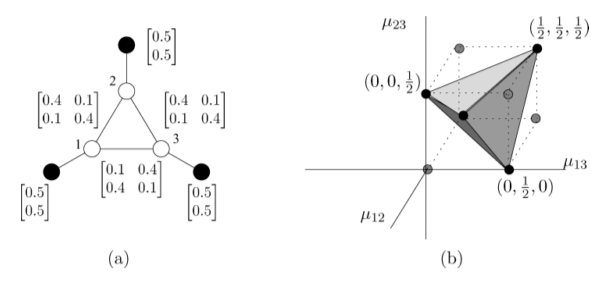
\includegraphics[width=.9\linewidth]{figure/4-1.PNG}
    \caption{
        (a) 特定的伪边际:将式 (4.9) 参数设置为 $\beta_{12} = \beta_{23} = 0.4, \beta_{13} = 0.1$,该伪边际满足局部一致性,不满足全局一致性。
        (b) 三点环图的边际多面体 $\mathbb{M}(C_3)$;
    }\label{fig:4-1}
\end{figure}

\subsection{贝特近似熵}

现在我们转向 Sum-product 算法的第二个变分成分,即对偶函数(负熵)的近似。
与边际多面体的外界 $\mathbb{L}(G)$ 一样,Bethe 熵近似也是基于树结构导出的。

对于一般的带环图上的 MRF 来说,负熵 $A^*$ —— 一个仅仅定义在均值参数 $\mu$ 上的函数 —— 明显缺乏封闭形式的表达式。
这种现象的一个重要例外是树结构上的 MRF,其熵可以分解为图上节点和边的局部熵。
为了导出这种分解形式,参考命题 4.1 的证明中因子分解式 (4.8),它将任意树结构的 MRF 分布分解为树上节点跟连边的边际分布 $\{\mu_s, s \in V\}$ 和 $\{\mu_{st}, (s, t) \in E\}$。
这些边际分布对应于正则过完备充分统计量 (3.34) 下的均值参数。
因此,对于树结构的 MRF,我们也能直接计算(负)对偶值 $-A^*(\mu)$,只需要计算分布 (4.8) 对应的熵 $H(p_{\mu})$ 即可。
使用 $\mathbb{E}_{\mu}$ 表示分布 (4.8) 下的期望,有:
\begin{align}
    H(p_{\mu}) = -A^*(\mu) &= \mathbb{E}_{\mu}[-\log p_{\mu}(X)] \nonumber \\
    &= \sum_{s \in V}H_s(\mu_s) - \sum_{(s, t) \in E}I_{st}(\mu_{st})
\end{align}
式中每个节点 $s \in V$ Singleton 的熵:
\begin{equation}
    H_s(\mu_s) := -\sum_{x_s \in \mathcal{X}_s}\mu_s(x_s)\log\mu_s(x_s)
\end{equation}
每条边 $(s, t) \in E$ 的互信息:
\begin{equation}
    I_{st}(\mu_{st}) := \sum_{(x_s, x_t) \in \mathcal{X}_s \times \mathcal{X}_t} \mu_{st}(x_s, x_t)\log\frac{\mu_{st}(xs, xt)}{\mu_s(x_s)\mu_t(x_t)}
\end{equation}
因此,对于树结构的图来说,对偶函数 $A^*$ 能够表达为一种精确且容易计算的均值参数 $\mu$ 的函数形式。

有了以上背景,带环图 MRF 的熵的 Bethe 近似就很容易描述了:
它简单地假定分解式 (4.11) 是带环图的一个合理近似。
根据这个假设,Bethe 近似熵可以表示为:
\begin{equation}
    -A^*(\mu) \approx H_{Bethe}(\tau) := \sum_{s \in V}H_s(\tau_s) - \sum_{(s, t) \in E}I_{st}(\tau_{st}).
\end{equation}
近似 (4.14) 可以用于任何一组属于 $\mathbb{L}(G)$ 的伪边际 $\{\tau_s, s \in V\}$ 以及 $\{\tau_{st}, (s, t) \in E\}$,这是 Sum-product 算法推导的核心条件。
因此,我们在符号上有意地将表示精确边际的 $\mu$ 换到了表示伪边际的 $\tau$。

Yedidia et al. 曾使用过一种不同于式 (4.14) 的 Bethe 近似熵,其实质是将互信息展开:$I_{st}(\tau_{st}) = H_s(\tau_s) + H_t(\tau_t) - H_{st}(\tau_{st})$,其中 $H_{st}$ 为伪边际 $\tau_{st}$ 的联合熵。
运用上述代换再经过简单的代数运算可得:
\begin{equation}
    H_{Bethe}(\tau) = -\sum_{s \in V}(d_s-1)H_s(\tau_s) + \sum_{(s, t) \in E}H_{st}(\tau_{st}), 
\end{equation}
式中 $d_s$ 代表节点 $s$ 的邻居数目(也就是节点 $s$ 的度)。
但是,对称形式的 (4.14) 在后续推断中是最自然的。

\subsection{贝特变分问题与和积算法}

我们现在已经具备了从定理 3.4 中的变分原理 (3.45) 中构建 Bethe 近似的两个原材料:
\begin{itemize}
    \item 满足局部一致性的伪边际 (4.7) 集合 $\mathbb{L}(G)$,其作为边际多面体 $\mathbb{M}(G)$ 的凸多面体外界;
    \item Bethe 熵 (4.14),其作为精确对偶函数 $A^*(\tau)$ 的近似。
\end{itemize}
组合两者即可得到 Bethe 变分问题(Bethe Variational Problem,BVP):
\begin{equation}
    \max_{\tau \in \mathbb{L}(G)}\left\{\langle\theta, \tau\rangle + \sum_{s \in V}H_s(\tau_s) - \sum_{(s, t) \in E}I_{st}(\tau_{st})\right\}.
\end{equation}

应当指出的是,这个问题具有一个非常简单的结构:
成本函数是显式给出的并且可微,约束集合 $\mathbb{L}(G)$ 是一个由少量约束决定的多面体。
给定这个特殊的结构,很容易想到优化问题 (4.16) 会有一个相对简单的求解算法,Sum-product 算法就是其中之一。

为了给出变分问题 (4.16) 与 Sum-product 算法之间的联系,令 $\lambda_{ss}$ 为归一化约束 $C_{ss}(\tau) = 0$ 的 Lagrange 乘子,其中:
\begin{equation}
    C_{ss}(\tau) := 1 - \sum_{x_s}\tau_s(x_s)
\end{equation}
此外,对每条边的每个方向 $s \rightarrow s$ 以及每个状态 $x_s \in \mathcal{X}_s$,定义如下约束函数:
\begin{equation}
    C_{ts}(x_s; \tau) := \tau_s(x_s) - \sum_{x_t}\tau_{st}(x_s, x_t),
\end{equation}
并且令 $\lambda_{ts}(x_s)$ 为约束 $C_{ts}(x_s; \tau) = 0$ 的 Lagrange 乘子。
这些 Lagrange 乘子与 Sum-product 消息联系紧密,事实上有 $M_{ts}(x_s) \propto \exp(\lambda_{ts}(x_s))$。

接下来考虑 Bethe 变分问题 (4.16) 的 Lagrangian:
\begin{align}
    \mathcal{L}(\tau, \lambda; \theta) := &\langle\theta, \tau\rangle + H_{Bethe}(\tau) + \sum_{s \in V}\lambda_{ss}C_{ss}(\tau) \nonumber \\
    & + \sum_{(s, t) \in E}\left[\sum_{x_s}\lambda_{ts}(x_s)C_{ts}(x_s; \tau) + \sum_{x_t}\lambda_{st}(x_t)C_{st}(x_t; \tau)\right].
\end{align}
依据上述定义,Yedidia et al. 给出了 Sum-product 算法与 BVP 的精确关系:

\begin{tcolorbox}
\begin{prop}[Sum-product 算法与 Bethe 问题]
    Sum-product 的消息更新机制是解决 Bethe 变分问题的一种 Lagrangian 方法:
    \begin{itemize}
        \item[(a)] 对于任意图 $G$,Sum-product 算法得到的任何不动点都给出一对 $(\tau^*, \lambda^*)$ 满足:
            \begin{equation}
                \nabla_{\tau}\mathcal{L}(\tau^*, \lambda^*; \theta) = 0, \quad \nabla_{\lambda}\mathcal{L}(\tau^*, \lambda^*; \theta) = 0.
            \end{equation}
        \item[(b)] 对于树结构的 MRF,Lagrangian 方程 (4.20) 有且仅有一个解 $(\tau^*, \lambda^*)$,其中 $\tau^*$ 的元素符合 MRF 精确的 Singleton 与 Pairwise 边际分布。
            此外,BVP 的最优值等价于累积函数 $A(\theta)$。
    \end{itemize}
\end{prop}
\end{tcolorbox}

\begin{tcolorbox}
\textbf{引注 4.1} 
    应当指出的是 Lagrangian 公式 (4.19) 是有所保留的,因为它只为归一化约束 $C_{ss}$ 与边际约束 $C_{ts}$ 配置了 Lagrange 乘子,而对非负性约束则采取了隐式处理。
    然而根据命题 4.2(a),Bethe 变分问题的任何严格正的最优解 $\tau^*$ 都必须满足 Lagrangian 条件 (4.20)。
    根据 Bertsekas 的工作,如果 $\lambda^*$ 是 BVP 的 Lagrange 乘子向量,那么最优解 $\tau^*$ 一定在正象限 $\tau \geq 0$ 最大化 Lagrangian $\mathcal{L}(\tau, \lambda^*)$。
    如果最优解 $\tau^*$ 严格正,那么 Lagrangian 最优性的一个必要条件就是 0 梯度条件 $\nabla_{\tau}\mathcal{L}(\tau^*, \lambda^*) = 0$。
    此外,对于为任意状态都分配了严格正质量的图模型(例如有限 $\theta$ 指数族形式的图模型)而言,Sm-product 算法传递的“消息”严格大于 0,因此也一定存在一个严格正的最优解 $\tau^*$。
    在这种情况下,命题 4.2(a) 保证了任意满足 Lagrangian 条件的 Sum-product 不动点都是 Bethe 变分问题的最优解。
    对于具有部分 0 质量状态的图模型而言则需要考虑另外的条件来保证不动点的最优性;
    详情可参见 Yedudua et al. 的工作。
\end{tcolorbox}

\analysis[证明]
(a) 部分的证明:计算偏导数 $\nabla_{\tau}\mathcal{L}(\tau; \lambda)$ 并让它等于 0 可得:
\begin{subequations}
\begin{align}
    \log\tau_s(x_s) &= \lambda_{ss} + \theta_s(x_s) + \sum_{t \in N(s)}\lambda_{ts}(x_s), \\
    \log\frac{\tau_{st}(x_s, x_t)}{\tilde{\tau}_s(x_s)\tilde{\tau}_t(x_t)} &= \theta_{st}(x_s, x_t) - \lambda_{ts}(x_s) - \lambda_{st}(x_t), 
\end{align}
\end{subequations}
其中 $\tilde{\tau}_s(x_s) := \sum_{x_t}\tau(x_s, x_t)$。
条件 $\nabla_{\lambda}\mathcal{L}(\tau; \lambda) = 0$ 等价于 $C_{ts}(x_s; \tau) = 0$ 以及 $C_{ss}(\tau) = 0$。
利用式 (4.21a) 以及边际条件 $C_{ts}(x_s; \tau) = 0$ 将式 (4.21b) 改写为:
\begin{align}
    \log\tau_{st}(x_s, x_t) &= \lambda_{ss} + \lambda_{tt} + \theta_{st}(x_s, x_t) + \theta_s(x_s) + \theta_t(x_t) \nonumber \\
    & + \sum_{u \in N(s)/t}\lambda_{us}(x_s) + \sum_{u \in N(t)/s}\lambda_{ut}(x_t).
\end{align}
为了建立与 Sum-product 算法的准确联系,我们为每条有向边 $t \rightarrow s$ 定义一个 $r_s$ 维的“消息”向量
\begin{equation*}
    M_{ts}(x_s) = \exp(\lambda_{ts}(x_s)), \quad \forall x_s \in \{0, 1, \cdots, r_s-1\}
\end{equation*}
使用这种记号式 (4.21a) 可以改写为:
\begin{equation}
    \tau_s(x_s) = \kappa\exp(\theta_s(x_s))\prod_{t \in N(s)}M_{ts}(x_s).
\end{equation}
式 (4.22) 可以改写为:
\begin{align}
    \tau_{st}(x_s, x_t) &= \kappa'\exp(\theta_{st}(x_s, x_t) + \theta_s(x_s) + \theta_t(x_t)) \nonumber \\
    &= \times \prod_{u \in N(s)/t}M_{us}(x_s) \prod_{u \in N(t)/s}M_{ut}(x_t).
\end{align}
式中 $\kappa, \kappa'$ 是依赖于 $\lambda_{ss}, \lambda_{tt}$ 的正常数,用于保证伪边际的归一化条件。
注意 $\tau_s$ 以及 $\tau_{st}$ 被定义为非负的。

综上,我们需要调整 Lagrange 乘子或者消息以使得每条边都满足边际约束 $\sum_{x_t}\tau_{st}(x_s, x_t) = \tau_s(x_s)$。
根据式 (4.23) 和 (4.24) 可得:
\begin{equation}
    M_{ts}(x_s) \propto \sum_{x_t}\left[\exp\{\theta_{st}(x_s, x_t)+\theta_t(x_t)\}\prod_{u \in N(t)/s}M_{ut}(x_t)\right], 
\end{equation}
上式与 Sum-product 的更新式 (2.9) 等价。
通过上述构造可以证明,式 (4.25) 更新得到的任何不动点 $M^*$ 都确定了一对 $(\tau^*, \lambda^*)$ 满足驻点条件 (4.20)。

\begin{note}
    译者经过计算给出的关系式与 (4.21) 不同:
    \begin{align*}
        \frac{\partial \mathcal{L}}{\partial \tau_s(x_s)} &= \theta_s(x_s) - \log\tau_s(x_s) - \lambda_{ss} + \sum_{t \in N(s)}\lambda_{ts}(x_s) \\
        &= 0 \\
        \Rightarrow \log\tau_{s}(x_s) &= \theta_s(x_s) - \lambda_{ss} + \sum_{t \in N(s)}\lambda_{ts}(x_s) \\
        \frac{\partial \mathcal{L}}{\partial \tau_{st}(x_s, x_t)} &= \theta_{st}(x_s, x_t) - \log\frac{\tau_{st}(x_s, x_t)}{\tau_s(x_s)\tau_t(x_t)} - 1 - \lambda_{ts}(x_s) - \lambda_{st}(x_t) \\
        &= 0 \\
        \Rightarrow \log\frac{\tau_{st}(x_s, x_t)}{\tau_s(x_s)\tau_t(x_t)} &= \theta_{st}(x_s, x_t) -1 - \lambda_{ts}(x_s) - \lambda_{st}(x_t)
    \end{align*}
    因此,式 (4.22) 也有不同:
    \begin{align*}
        \log\tau_{st}(x_s, x_t) &= -1 - \lambda_{ss} - \lambda_{tt} + \theta_{st}(x_s, x_t) + \theta_s(x_s) + \theta_t(x_t) \\
        & + \sum_{u \in N(s)/t}\lambda_{us}(x_s) + \sum_{u \in N(t)/s}\lambda_{ut}(x_t).
    \end{align*}
    然而在后续推导中这些问题均隐含在归一化常数 $\kappa$ 与 $\kappa'$ 里,因此形式上的差异消失了。
\end{note}

(b) 部分的证明参见附录 B.4。
\qed

Sum-product 算法与 Bethe 变分原理之间的这种联系可以导出许多重要结论。
首先,它为在带环图上应用 Sum-product 算法提供了理论基础,也就是采用一种迭代的方式尝试解出满足 Lagrangian 条件的解。
然而应当注意的是,Sum-product 与 Bethe 问题之间的这种联系并未保证 Sum-product 迭代可以在带环图上收敛。
实际上,算法能否收敛取决于势强度(Potential Strengths)以及图的拓扑结构。
标准的消息传递机制中,每个节点都是并行应用式 (4.25) 的。
其他更为全局性的消息传递机制也是可行的,这些机制也可以用在例如纠错编码等特定应用中。
Tatikonda 和 Jordan 在无限展开的计算树(Infinitely Unwrapped Computation Tree)上建立了并行更新的收敛条件和 Gibbs 测度之间的联系,从而表明了由 Gibbs 测度的经典唯一性条件可以得到收敛的充分条件(也就是 Dobrushin 条件或者 Simon 条件)。
在之后的工作中,其他研究人员使用了各种类型的收缩论点来获得更清晰的不动点的收敛条件和唯一性条件。
对于某种程度的弱势(Suitably Weak Potentials),Dobrushin 条件和相关的压缩参数可以保证更新的收敛性,也就保证了相关不动点的唯一性。
另一些工作也在探索 Sum-product 的替代方案,这些方案可以保证收敛,只不过需要增加计算成本。
但是,除了树和某些特殊情况,Bethe 变分问题通常是非凸的,因为 $H_{Bethe}$ 并不是凹的。
因此即使使用了收敛算法也不能保证收敛到全局最优值,经常会收敛到局部最优。

对于每个 $\theta \in \mathbb{R}^d$,令 $A_{Bethe}(\theta)$ 代表 Bethe 变分问题 (4.16) 的最优值。
命题 4.2(b) 表明对于任意的树结构问题,有 $A_{Bethe}(\theta) = A(\theta)$,这个等式对所有 $\theta \in \mathbb{R}^d$ 成立。
在这种等价性下很容易自然联想到对于一般图来说 $A_{Bethe}(\theta)$ 和累积函数 $A(\theta)$ 之间的关系。
一般而言,Bethe 值 $A_{Bethe}(\theta)$ 只是累积函数 $A(\theta)$ 的一个简单近似。
与第 5 节会讨论的平均场方法不同,$A_{Bethe}(\theta)$ 并不保证是累积函数的一个下界。
第 7 节中将会花费更长的篇幅来讨论由 Wainwright et al. 导出的 Convexified 形式的 Bethe 变分原理,它可以为任意图模型提供关于累积函数上界的估计。
另一方面,Sudderth et al. 发现对于某些有意思的图模型来说 $A_{Bethe}(\theta)$ 也确实是累积函数 $A(\theta)$ 的一个下界。
这些模型一般都鼓励随机变量彼此之间趋于一致,在计算机视觉与空间统计等应用中比较常见。
相应的下界性质跟 Bethe 近似与循环级数展开(Loop Series Expansions)之间的联系关系密切,4.1.6 小节将会对这一点进行讨论。

Bethe 问题与 Sum-product 算法之间的联系所导出的另一个重要结论是,通过逐步更好地逼近熵函数和边际多面体的外边界可以提出许多改进普通 Sum-product 算法的方法。
4.2 节将会讨论一类这样的广义 Sum-product 算法。

\subsection{贝特问题与和积算法的误差}

这一小节我们讨论 Sum-product 算法的误差。
从变分的角度来看,误差来源于构造 Bethe 变分原理的两个近似:

\begin{itemize}
    \item[(1)] 采用多面体外界 $\mathbb{L}(G)$ 代替了边际多面体 $\mathbb{M}(G)$,
    \item[(2)] 采用 Bethe 熵 $H_{Bethe}$ 作为均值参数精确熵函数的近似。
\end{itemize}

我们先考虑 Bethe 熵近似以及它带来的潜在误差:

\begin{tcolorbox}
\begin{exam}[$H_{Bethe}$ 的误差]

考虑四个节点的全连接图 $K_4$,Singleton 与 Pairwise 的边际分布为:
\begin{subequations}
\begin{align}
    \mu_s(x_s) &= [0.5, 0.5] &\text{for } s = 1, 2, 3, 4 \\
    \mu_{st}(x_s, x_t) &= \begin{bmatrix}
        0.5 & 0 \\
        0 & 0.5
    \end{bmatrix} &\forall (s, t) \in E.
\end{align}
\end{subequations}
这些边际满足全局一致性,事实上,在状态 $(0, 0, 0, 0)$ 与 $(1, 1, 1, 1)$ 上各自分配 0.5 的概率就可以导出这些边际。
Bethe 近似熵的计算很简单,每个 Singleton 的熵为 $H_s(\mu_s) = \log 2$,每条边的互信息为 $I_{st}(\mu_{st}) = \log 2$,所以 Bethe 熵为:
\begin{equation*}
    H_{Bethe}(\mu) = 4\log 2 - 6\log 2 = -2\log 2 < 0,
\end{equation*}
显然不可能是一个真正的熵值。
事实上,这个例子的真熵值(或者说负对偶函数值)为 $-A^*(\mu) = \log 2 > 0$。

\end{exam}
\end{tcolorbox}

除了采用 $H_{Bethe}$ 作为负对偶函数的近似之外,Bethe 变分原理的误差还来自于将边际多面体 $\mathbb{M}(G)$ 放松到了一阶约束集合 $\mathbb{L}(G)$ 上。
如例 4.1 所示,3 个节点的环 $C_3$ 严格满足包含关系 $\mathbb{M}(C_3) \subseteq \mathbb{L}(C_3)$。
将例 4.1 的构造方法进行拓展可以证明包含关系 $\mathbb{M}(G) \subset \mathbb{L}$ 对于任何带环图 $G$ 都是严格成立的。
图 \ref{fig:4-2} 给出了 $\mathbb{M}(G)$ 和 $\mathbb{L}(G)$ 之间关系的一个理想化的示意图\footnote{
    应当指出的是这幅图也具有一定的误导性,因为在那上面 $\mathbb{L}(G)$ 比 $\mathbb{M}(G)$ 具有更多的切面和顶点。
    事实上多面体 $\mathbb{L}(G)$ 的切面数目更少而顶点数目更多,但这种特性在二维图上很难表示出来。
}:两个集合都是多面体,同时对于任意带环图来说,$\mathbb{M}(G)$ 总是严格含于外边界 $\mathbb{L}(G)$。

\begin{figure}[htbp]
    \centering
    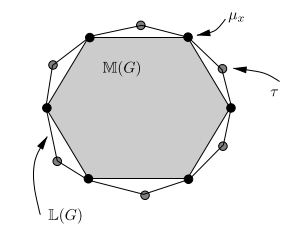
\includegraphics[width=.5\linewidth]{figure/4-2.PNG}
    \caption{
        边际多面体 $\mathbb{M}(G)$ 与外边界 $\mathbb{L}(G)$ 之间关系的理想化示意图。
        集合 $\mathbb{L}(G)$ 永远是 $\mathbb{M}(G)$ 的一个外边界,而对于任意带环图 $G$ 来说包含关系 $\mathbb{M}(G) \subset \mathbb{L}(G)$ 都严格成立。
        两个集合都是多面体,所以都能够用有限数目的极值点(Extreme Points)构成的凸包(Convex Hull)或者有限数目的半空间(Half-spaces)也就是切面(Facets)进行表示。
    }\label{fig:4-2}
\end{figure}

这两个集合都是多面体,因此可以表示为有限数目的极值点的凸包,或者是有限数目的半空间也就是切面的交集。
令 $\phi$ 代表标准过完备表示 (3.34) 指示函数所构成的全向量,边际多面体可以表示为凸包 $\mathbb{M}(G) = conv\{\phi(x)| x \in \mathcal{X}^m\}$。
由于指示函数为 $\{0, 1\}$ 取值,它的所有极值点都是由 $\{0, 1\}$ 元素构成,其实质为某些 $x \in \mathcal{X}^m$ 的特征量 $\mu_x := \phi(x)$,这样的极值点一共有 $|\mathcal{X}^m|$ 个。
然而除了树结构的图之外,$\mathbb{M}(G)$ 切面的数目一般是未知的,对于简单如 Ising 模型等例子也是如此。
而且切面的数目随着图的规模的增长一定是超多项式的(Super-polynomial),除非在计算复杂度方面某些被广泛认可的猜想实际是错的。

另一方面,多面体 $\mathbb{L}(G)$ 具有多项式数目的切面,对于任意图模型来说都有上界 $\mathcal{O}(rm+r^2|E|)$。
$\mathbb{L}(G)$ 相比 $\mathbb{M}(G)$ 具有更多的极值点,因为除了所有的整点(Integral Extreme Points)$\{\mu_x, x \in \mathcal{X}^m\}$ 之外,它还包括其他一些具有分数元素的极值点 $\tau \in \mathbb{L}(G)/\mathbb{M}(G)$。
8.4 节对整数极值点和分数极值点进行了进一步的讨论。
除了树和其他一些小规模的实例外,$\mathbb{L}(G)$ 的极值点数目一般也是未知的。

$\mathbb{M}(G)$ 与 $\mathbb{L}(G)$ 之间的严格包含关系 —— 以及后者在 Bethe 变分问题 (4.16) 中的基本角色 —— 引出了以下问题:
Bethe 变分问题的解会总是落入 $\mathbb{M}(G)/\mathbb{L}(G)$ 的间隔(Gap)中吗?
乐观主义者会希望这些点能通过某种方式被排除在 Bethe 变分问题的最优解之外。
不幸的是,这种乐观主义想法被证明是具有误导性的。
事实上,对于 $\mathbb{L}(G)$ 中的每一个元素 $\tau$ 都可以构造一个分布 $p_{\theta}$,使得 $\tau$ 满足 Sum-product 的不动点所定义的消息。
为了理解这件事情,我们接下来讨论 Sum-product 的重参数化解释(Reparameterization Interpretation)。

\subsection{贝特最优与重参数化}

2.5.2 小节描述的联合树算法可以从如下角度进行理解:
将某个图上团的势函数集合作为输入,联合树算法输出相同分布的因子分解结果,这些因子就是联合树上的团集和分割集上的局部边际。
在树结构的特殊情况下,因子是各个节点以及各个连边上的边际,如式 (4.8) 所示。
事实上,树的 Sum-product 算法可以被理解为进行这种参数化的有效方法。

同样的解释也适用于任意带环图:
更准确地说,Sum-product 算法的任何不动点 —— 甚至更普遍地说,Bethe 变分原理的任意局部最优点 —— 都指定了原始分布 $p_{\theta}$ 的一种重参数化形式。
我们将这一事实总结为如下命题:

\begin{tcolorbox}
\begin{prop}[Bethe 近似的重参数化性质]

令 $\tau^* = (\tau_s^*, s \in V; \tau_{st}^*, (s, t) \in E)$ 表示由分布 $p_{\theta}$ 定义的 Bethe 变分原理的任意最优点。
则根据该不动点定义的如下分布:
\begin{equation}
    p_{\tau^*}(x) := \frac{1}{Z(\tau^*)}\prod_{s \in V}\tau_s^*(x_s)\prod_{(s, t) \in E}\frac{\tau_{st}^*(x_s, x_t)}{\tau_s^*(x_s)\tau_t^*(x_t)},
\end{equation}
就是原始分布 $p_{\theta}$ 的一种重参数化形式 —— 也就是说对于所有 $x \in \mathcal{X}^m$,都有 $p_{\tau^*}(x) = p_{\theta}(x)$。

\end{prop}
\end{tcolorbox}

应当注意的是,这种重参数化仅仅在由指示函数 (3.34) 定义的过完备表示下的指数族中有效。
重参数化 (4.27) 实际上是树结构分解 (4.8) 的一个类比,只不过应用在带环图上。
与树结构情况不同的是,归一化常数 $Z(\tau^*)$ 一般并不等于 1。
尽管联合树定理保证了任何树结构可以进行重参数化,但是对于一般的图而言,即使重参数化存在也是不容易直接看出来的。
事实上,每个图至少有一个这种形式的重参数化表示,有些图可能有多个,例如对于任何 BVP 具有多个最优解的问题就是如此。
此外,重参数化观点为 $p_{\theta}(x)$ 的精确边际 $\mu_s$ 与由 Sum-product 算法给出的近似 $\tau_s^*$ 之间的差异 所造成的近似误差提供了一些见解。
实际上,应用式 (4.27) 可以推导出 Sum-product 算法中的误差的精确表达式,以及可计算的误差界,这些工作由 Wainwright et al. 完成。

我们接下来借助重参数化表征 (4.27) 为 $\mathbb{L}(G)$ 中的任何由 Sum-product 算法得到的不动点对应的伪边际 $\tau$ 指定相应的分布 $p_{\theta}$。
以下面这个例子进行说明。

\begin{tcolorbox}
\begin{exam}[“戏弄” Sum-product 算法]

我们还是考虑使 Sum-product 算法不精确的最简单的图,也就是三个节点的环(同例 4.1)。
考虑候选边际分布 $(\tau_s, s \in V)$ 以及 $(\tau_{st}, (s, t) \in E)$,并按图 \ref{fig:4-1}(a) 进行配置,$\beta_{12} = \beta_{23} = 0.4, \beta_{13} = 0.1$。
如例 4.1 中的讨论,这种配置所构建的伪边际 $\tau$ 是 $\mathbb{L}(G)$ 中的元素,但不是 $\mathbb{M}(G)$ 中的元素,因此也就无法从任何满足全局一致性的分布中导出。

现在让我们证明,对于图上一个经过适当选择的分布 $p_{\theta}$,Sum-product 算法是如何被“戏弄”从而收敛到伪边际向量 $\tau$ 上的。
使用正则过完备表示 (3.34),考虑如下形式的正则参数:
\begin{subequations}
\begin{align}
    \theta_s(x_s) &:= \log\tau_s(x_s) = \log [0.5, 0.5] &\forall s \in V, \\
    \theta_{st}(x_s, x_t) &:= \log\frac{\tau_{st}(x_s, x_t)}{\tau_s(x_s)\tau_t(x_t)} & \nonumber \\
    &= \log 4\begin{bmatrix}
        \beta_{st} & 0.5-\beta_{st} \\
        0.5-\beta_{st} & \beta_{st}
    \end{bmatrix} &\forall (s, t) \in E
\end{align}
\end{subequations}
式中我们采用了式 (4.2) 的简写。
在上面这些正则参数的配置下,假设我们在 MRF $p_{\theta}(x)$ 上应用 Sum-product 算法,并进行均匀初始化 $M_{ts}(x_s) \propto [0.5, 0.5]$。
根据式 (4.25) 可知,这种均匀初始化 $M$ 已经为 Sum-product 定义了一个不动点。
此外,如果我们计算由 $M$ 和 $\theta$ 指定的相应伪边际,就会发现结果就是之前定义的 $\tau_s$ 以及 $\tau_{st}$。
综上,当 Sum-product 算法应用于由式 (4.28) 所定义的正则参数相应的分布 $p_{\theta}$ 上时,会输出伪边际 $\tau$ 作为真实边际的估计。

读者可能会反对这样的初始化方法,也就是一开始就将消息初始化在不动点上会导致算法排除其他可能的不动点。
然而根据已有的一些工作,对于任何最多只有一个环路的离散指数族 MRF 来说,Sum-product 具有唯一的不动点,且一定收敛到该不动点。
因此,我们构造的不动点 (4.28) 是这个问题的唯一不动点,算法从消息的任意初始化开始都会收敛到这个不动点上。

\end{exam}
\end{tcolorbox}

更一般的说,上述例子中展示的构造方法适用于 $\mathbb{L}(G)$ 中的任何内点\footnote{
    严格说来,它适用于相对内部的元素,因为如过完备表示 (3.34) 所述,集合 $\mathbb{L}(G)$ 不是全维度的(Full-dimensional),因此有一个空的内部(Empty Interior)。
}。因此,对于所有的伪边际 $\tau \in \mathbb{L}(G)$,包括那些不满足全局一致性的,都存在分布 $p_{\theta}$ 可以使得 $\tau$ 从 Sum-product 的不动点中导出。

\begin{note}
    译者对脚注 (4) 产生了莫大的疑问。
    $\mathbb{L}(G)$ 为什么会有个“空的内部”?
    它不是一个简单的“实心”的凸多面体吗?
\end{note}

\subsection{贝特与循环级数展开}

本小节我们讨论 Chertkov 与 Chernyak 的循环级数展开。
这些展开项提供了累积函数作为项和的精确表示,其中第一项就是 Bethe 近似 $A_{Bethe}(\theta)$,并且可以通过添加所谓的循环修正(Loop Corrections)而得到高阶项。
他们为循环级数提供了两种推导:第一种对二元变量的 Fourier 表示应用了三角恒等式,第二种是通过复变量辅助场得到的鞍点近似。
在本小节中我们采用一种更为直接的方式来导出循环级数,这种方法利用了命题 4.3 中给出的 Sum-product 不动点的重参数化特征。
尽管循环级数展开可以扩展到一般的因子图上,但考虑带有二元变量的成对 MRF —— 即例 3.1 中的 Ising 模型 —— 足以说明基本思想。
(因子图的推导可以参见 Sudderth et al. 的工作。)

在揭示结论之前,我们先做一些初步的定义。
给定一个无向图 $G = (V, E)$ 以及连边 $E$ 的一个子集 $\tilde{E} \subseteq E$,令 $G(\tilde{E})$ 表示与连边集合 $\tilde{E}$ 与节点集合
\begin{equation}
    V(\tilde{E}) := \{t \in V| (t, u) \in \tilde{E} \quad \text{for some } u\}
\end{equation}
的一个子图。
对于任意节点 $s \in V$,我们定义其与 $\tilde{E}$ 相关的度为
\begin{equation}
    d_s(\tilde{E}) := \{t \in V| (s, t) \in \tilde{E}\}.
\end{equation}
根据 Chertkov 与 Chernyak 的工作,我们定义广义环(Generalized Loop)的概念为一个子图 $G(\tilde{E})$,其每个节点 $s \in V$ 的度均满足 $d_s(\tilde{E}) \neq 1$。
换句话说,对于每个节点 $s \in V$,它要么 $d_s(\tilde{E}) = 0$ 从而不属于 $G(\tilde{E})$,要么 $d_s(\tilde{E}) \geq 2$。
图 \ref{fig:4-3} 给出了广义环的示意说明。
应当指出的是,无环图(也就是树或者森林图)是没有任何广义环的。

\begin{figure}[htbp]
    \centering
    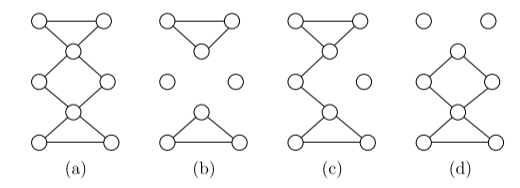
\includegraphics[width=.9\linewidth]{figure/4-3.PNG}
    \caption{
        广义环示意。
        (a) 原始图。
        (b)-(d) 与 (a) 中原始图相关的几个广义环。
        在这个特定的例子中,原始图自身也是一个自己的广义环。
    }\label{fig:4-3}
\end{figure}

考虑二元变量的成对 MRF —— 也就是 Ising 模型 (3.8) —— 的一个 BP 不动点。
对于二元变量 $X_s \in \{0, 1\}$,与 BP 不动点相关的 Singleton 和 Edgewise 的伪边际可以参数化为
\begin{equation}
    \tau_s(x_s) = \begin{bmatrix}
        1 - \tau_s \\
        \tau_s
    \end{bmatrix}, \quad \tau_{st}(x_s, x_t) = \begin{bmatrix}
        1 - \tau_s - \tau_t + \tau_{st} & \tau_t - \tau_{st} \\
        \tau_s - \tau_{st} & \tau_{st}
    \end{bmatrix}
\end{equation}
通过一些简单的计算可以将 $\mathbb{L}(G)$ 用以下四个不等式进行描述:
\begin{equation*}
    \tau_{st} \geq 0, 1-\tau_s-\tau_t+\tau_{st} \geq 0, \tau_s-\tau_{st} \geq 0, \tau_t-\tau_{st} \geq 0,
\end{equation*}
这四个不等式对每条边 $(s, t) \in E$ 都成立。
有关 Ising 模型的均值参数的讨论可以参见例 3.8。

使用这个参数表示,我们为每条边 $(s, t) \in E$ 定义边权重(Edge Weight)
\begin{equation}
    \beta_{st} := \frac{\tau_{st}-\tau_s\tau_t}{\tau_s(1-\tau_s)\tau_t(1-\tau_t)}
\end{equation}
将其自然拓展到子图权重(Subgraph Weight)$\beta_{\tilde{E}} := \prod_{(s, t) \in \tilde{E}}\beta_{st}$。
有了这些定义,我们可以提出以下命题:

\begin{tcolorbox}
\begin{prop}

考虑一个二元变量的成对 MRF (3.8),令 $A_{Bethe}(\theta)$ 表示自由能 (4.16) 在 BP 不动点 $\tau = (\tau_s, s \in V; \tau_{st}, (s, t) \in E)$ 处取得的最优值。
累积函数 $A(\theta)$ 等价于下列循环级数展开:
\begin{equation}
    A(\theta) = A_{Bethe}(\theta) + \log\left\{1+\sum_{\emptyset\neq\tilde{E}\subseteq E}\beta_{\tilde{E}}\prod_{s \in V}\mathbb{E}_{\tau_s}[(X_s - \tau_s)^{d_s(\tilde{E})}]\right\}.
\end{equation}

\end{prop}
\end{tcolorbox}

在证明命题 4.4 之前,我们先暂停一下做一些注释。
根据定义我们有
\begin{align}
    \mathbb{E}_{\tau_s}[(X_s - \tau_s)^d] &= (1-\tau_s)(-\tau_s)^d + \tau_s(1-\tau_s)^d \nonumber \\
    &= \tau_s(1-\tau_s)[(1-\tau_s)^{d-1}+(-1)^d(\tau_s)^{d-1}], 
\end{align}
其实质是一个参数为 $\tau_s \in [0, 1]$ 的 Bernoulli 变量的 $d$ 阶中心矩。
因此,对于至少有一个节点 $s \in V$ 满足 $d_s(\tilde{E}) = 1$ 的连边子集 $\tilde{E} \subseteq E$,其在展开式 (4.33) 中相应的项被消除了。
所以,只有广义环 $\tilde{E}$ 在展开式 (4.33) 中保留下来。
与这些广义环相关的项定义了对累积函数的 Bethe 近似 $A_{Bethe}(\theta)$ 的修正。
此外,树结构的图不包含任何非平凡的广义环,这提供了树结构图的 Bethe 近似实际上十分精确的另一种证明。

循环展开的第一项 $A_{Bethe}(\theta)$ 很容易从任何 BP 不动点计算出来,因为它只对应于 Bethe 自由能的最优值 (4.16)。
然而,整个循环修正序列的显式计算 —— 也就是对累积函数的精确计算 —— 对于一般的图模型来说仍旧困难。
例如,任何 $n \geq 5$ 个节点的全连通图都有超过 $2^n$ 个广义环。
在某些情况下,对一小组重要的循环修正进行计算可能会提高对配分函数的近似,或者为 LDPC 编码的边际提供更加精确的近似。

\analysis[命题 4.4 的证明]
使用指示函数进行的正则过完备参数化 (3.34) 是过完备的,因此有许多不同的正则参数向量 $\theta \neq \theta'$ 对应相同的分布 $p_{\theta} = p_{\theta'}$。
然而,循环级数展开 (4.33) 左侧与右侧的区别对于任意 $\theta$ 都是相同的,因为变换 $\theta \rightarrow \theta'$ 仅仅将 $A(\theta)$ 与 $A_{Bethe}(\theta)$ 都偏移了同一个常数。
因此,我们只需要证明一种参数化形式的循环级数展开即可;
特别地,我们选择使用由任意 BP 不动点给出的重参数化形式下的正则参数:
\begin{equation}
    \tilde{\theta} = \log\tau_s(x_s), \quad \tilde{\theta}_{st}(x_s, x_t) = \log\frac{\tau_{st}(x_s, x_t)}{\tau_s(x_s)\tau_t(x_t)}.
\end{equation}
在这个重参数化形式下,通过简单计算即可知 $A_{Bethe}(\tilde{\theta}) = 0$。
因此,我们只需要证明在这个重参数化 (4.35) 条件下等式
\begin{equation}
    A(\tilde{\theta}) = \log\left\{1+\sum_{\emptyset\neq\tilde{E}\subseteq E}\beta_{\tilde{E}}\prod_{s \in V}\mathbb{E}_{\tau_s}[(X_s-\tau_s)^{d_s(\tilde{E})}]\right\}
\end{equation}
成立即可。
使用表示 (4.31),通过简单的计算可知
\begin{equation}
    \frac{\tau_{st}(x_s, x_t)}{\tau_s(x_s)\tau_t(x_t)} = 1 + \beta_{st}(x_s-\tau_s)(x_t-\tau_t).
\end{equation}
根据 $\tilde{\theta}$ 的定义,我们有
\begin{equation*}
    \exp(A(\tilde{\theta})) = \sum_{x \in \{0, 1\}^m}\prod_{s \in V}\tau_s(x_s)\prod_{(s, t) \in E}\frac{\tau_{st}(x_s, x_t)}{\tau_s(x_s)\tau_t(x_t)}.
\end{equation*}
令 $\mathbb{E}$ 表示乘积分布 $\tau_{fact}(x) := \prod_s\tau_s(x_s)$ 下的期望。
考虑 (4.37) 式,我们有
\begin{align}
    \exp(A(\tilde{\theta})) &= \sum_{x \in \{0, 1\}^m}\prod_{s \in V}\tau_s(x_s)\prod_{(s, t) \in E}\frac{\tau_{st}(x_s, x_t)}{\tau_s(x_s)\tau_t(x_t)} \nonumber \\
    &= \mathbb{E}\left[\prod_{(s, t) \in E}(1+\beta_{st}(X_s-\tau_s)(X_t-\tau_t))\right].
\end{align}
对这个多项式进行展开并利用期望的线性性质,可以得到图中每个非空的连边子集 $\tilde{E} \subseteq E$ 对应的项:
\begin{equation}
    \exp(A(\tilde{\theta})) = 1 + \sum_{\emptyset\neq\tilde{E}\subseteq E}\mathbb{E}\left[\prod_{(s, t) \in \tilde{E}}\beta_{st}(X_s-\tau_s)(X_t-\tau_t)\right].
\end{equation}
之后,表达式 (4.36) 可以依据 $\tau_{fact}(x)$ 的独立性与 Bernoulli 变量的矩的标准公式得到。
计算过程中应当注意如果 $d_s(\tilde{E}) = 1$,那么就有 $\mathbb{E}[X_s-\tau_s] = 0$。
因此,每个广义环 $\tilde{E}$ 都会有一个循环校正。
\qed

命题 4.4 可以拓展到更加一般的因子图上。
此外,Sudderth et al. 的工作表明对于一类具有相互吸引作用的图模型来说,其 Bethe 值 $A_{Betha}(\theta)$ 实际上是真实累积函数 $A(\theta)$ 值的一个下界。

\section{菊池与基于超树的方法}

Bethe 变分原理 (4.16) 从两种不同的角度对精确变分原理 (3.45) 进行了近似。
首先对于一般图而言,Bethe 熵 (4.14) 仅仅是真实熵或者说负对偶函数的近似。
其次约束集合 $\mathbb{L}(G)$ 也是边际多面体 $\mathbb{M}(G)$ 的一个外边界,如图 \ref{fig:4-2} 所示。
从原理上来说,Bethe 变分原理可以通过对两者进行改进来提升近似效果。
本节主要考虑一种自然的拓展方法来对 Bethe 近似进行泛化,这些工作最开始是由 Yedidia et al. 提出的,之后也得到了其他研究者的拓展,对 Bethe 近似的两个成分都进行了改进。
这些方法的原始记录来源于统计物理文献,被称为簇变分方法(Cluster Variational Methods)。

从高一点的视角来看,Bethe 方法给出的近似是基于树结构的,这是联合树结构的一种特例。
那么一种自然的拓展策略就是考虑对更加复杂的联合树进行近似。
这些近似条件在超树(Hypertrees)的结构上很容易理解,因为超树就是联合树的表示方法之一。
因此,接下来我们介绍一些超图(Hypergraphs)和超树的必要背景。

\subsection{超图和超树}

超图 $G = (V, E)$ 是对图的一种泛化,包括节点集合 $V = \{1, \cdots, m\}$,以及超边(Hyperedges)集合 $E$,所谓的超边 $h$ 是指节点集合 $V$ 的一个特定子集。
这些超边构成了一个偏序集(Partially Ordered Set,Poset),这种偏序性质是由包含关系给出的。
当一条超边 $h$ 不被其他超边包含的时候,则称该超边 $h$ 为最大的(Maximal)。
根据这些定义,我们可以看到普通图就是超图的特例,其中每个最大超边由一对顶点构成,也就是普通图的一条普通边\footnote{
    我们这里的超边集合 $E$ 的定义与图论术语有一个小小的不同,对于超图(不是普通图),超边集合可以包含一个单独的节点 $\{s\}$ 作为一个元素。
}。

超图中有一种方便的图表示方法,那就是用超边图来表示,也就是采用有向边来表示包含关系,这样的表示称为偏序集图(Poset Diagram)。
图 \ref{fig:4-4} 给出了一些简单的超图示例。
任何普通图,也就是超图的特例,也可以用偏序集图的方式画出来。
例如,子图 (a) 展示了四节点单环的超图表示,子图 (b) 展示了一个非普通图的超图,它由两个大小为 3 的超边以及大小为 2 的交集组成,子图 (c) 是一个更加复杂的超图,我们之后会继续讨论这个超图。

\begin{figure}[htbp]
    \centering
    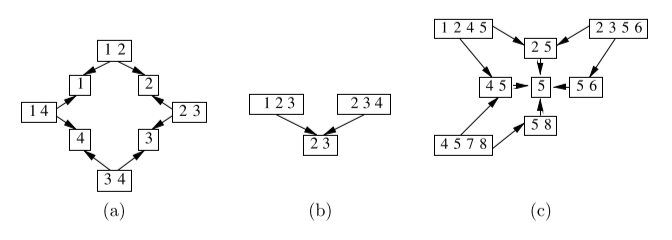
\includegraphics[width=.9\linewidth]{figure/4-4.PNG}
    \caption{
        超图的图表示。
        超边的节点子集用矩形表示,箭头则表示超边之间的包含关系。
        (a) 用超图表示的一个普通单环图。
        (b) 宽度为 2 的简单超树。
        (c) 宽度为 3 的一个更加复杂的超图。
    }\label{fig:4-4}
\end{figure}

超树,或者说无环超图,提供了一种方法来描述 2.5.2 小节中给出的联合树的概念。
特别地,如果超图可以使用最大超边和它们的交集给出一个联合树,那么这个超图就是无环的。
无环超图的宽度就是最大超边的大小减 1,我们将宽度为 $k$ 的由单个连通分量构成的无环超图称为 $k$ 阶超树(k-hypertree)。
例如,一个普通图的生成树是 1 阶超树,因为它的最大超边,也就是原始图中的一条普通边,大小都是 2。
再考虑图 \ref{fig:4-4}(c) 中的超图,显然这个超图等价于最大团为 $\{(1245), (4578), (2356)\}$,分割子为 $\{(25), (45)\}$ 的联合树。
因为最大超边的大小为 4,所以这个超图是一个宽度为 3 的超树。

\subsection{基于超树的因子化与熵的分解}

我们接下来给出联合树因子化 (2.12) 的另一种形式,并指出这种形式可以导致对熵的局部分解。
我们将超边集合 $E$ 看做是一个偏序集合,如附录 E.1 所描述的,每一个偏序集合都可以定一个 M\"obius 函数 $\omega: E \times E \rightarrow \mathbb{R}$。
使用边际集合 $\mu = (\mu_h, h \in E)$ 与超边集合进行关联,就能定义一个新的函数集合 $\varphi := (\varphi_h, h \in E)$ 如下:
\begin{equation}
    \log\varphi_h(x_h) := \sum_{g \subseteq h}\omega(g, h)\log\mu_g(x_g)
\end{equation}
根据以上定义以及 M\"obius 逆公式(参见附录 E.1 中的引理 E.1),边际可以表示为
\begin{equation}
    \log\mu_h(x_h) = \sum_{g \subseteq h}\log\varphi_g(x_g).
\end{equation}
这个公式为计算函数 $\varphi_g$ 提供了一种非常有用的递归方法,在下面会通过一个例子来进行说明。

函数 (4.40) 的意义在于为任何超树结构的图提供了一种非常简单的因子化方法。
特别地,对于具有包含最大超边之间交集的连边集合的超图来说,其上的分布具有如下因子分解:
\begin{equation}
    p_{\mu}(x) = \prod_{h \in E}\varphi_h(x_h; \mu)
\end{equation}
使用 $\varphi_h(x_h; \mu)$ 是为了强调 $\varphi_h$ 是边际 $\mu$ 的一个函数。
式 (4.42) 是著名的联合树分解 (2.12) 的另一种形式。
接下来我们通过一些例子加深理解。

\begin{tcolorbox}
\begin{exam}[超树的因子化]

(a) 首先假设超树为一个普通树,那么超边集合就是顶点集合与普通连边集合的并集。
将这个超边集合视为包含关系下的一个偏序集,那么其 M\:obius 函数具有如下形式:
对于所有超边 $g \in E$,有 $\omega(g, g) = 1$;
对于所有顶点 $s$ 以及普通连边 $\{s, t\}$,有 $\omega(\{s\}, \{s, t\}) = -1$;
另外对于所有不含于 $h$ 的 $g$,有 $\omega(g, h) = 0$。
因此,对于任何普通连边 $\{s, t\}$ 有:
\begin{equation*}
    \varphi_{st}(x_s, x_t) = \frac{\mu_{st}(x_s, x_t)}{\mu_s(x_s)\mu_t(x_t)}, 
\end{equation*}
而对于任何节点则有 $\varphi_s(x_s) = \mu_s(x_s)$。
因此在这种情况下,式 (4.42) 就可以化为式 (4.8) 中的树结构因子分解。

(b) 现在考虑一个更复杂一点的例子。
考虑由超边集合
\begin{equation*}
    E = \{(1245), (2356), (4578), (25), (45), (56), (58), (5)\}, 
\end{equation*}
给定的无环超图,如图 \ref{fig:4-4}(c) 所示。
相比计算偏序集的 M\"obius 函数,通过式 (4.41) 进行计算会更加方便。
由于表示符号的意义都比较明显,接下来我们略去对 $x$ 的显式表达,先计算 Singleton 函数 $\varphi_5 = \mu_5$,以及 Pairwise 函数 $\varphi_{25} = \mu_{25}/\mu_5$,其他 Pairwise 函数可以类比计算得到。
然后对 $h = (1245)$ 有
\begin{equation*}
    \varphi_{1245} = \frac{\mu_{1245}}{\varphi_{25}\varphi_{45}\varphi_5} = \frac{\mu_{1245}}{\frac{\mu_{25}}{\mu_5}\frac{\mu_{45}}{\mu_5}\mu_5} = \frac{\mu_{1245}\mu_5}{\mu_{25}\mu_{45}}.
\end{equation*}
通过类比计算也可以得到 $\varphi_{2356}$ 和 $\varphi_{4578}$ 的表达式。
把这些项集合起来就能得到密度 $p_{\mu}$ 的因子分解
\begin{align*}
    p_{\mu} &= \frac{\mu_{1245}\mu_5}{\mu_{25}\mu_{45}}\frac{\mu_{2356}\mu_5}{\mu_{25}\mu_{56}}\frac{\mu_{4578}\mu_5}{\mu_{45}\mu_{58}}\frac{\mu_{25}}{\mu_5}\frac{\mu_{45}}{\mu_5}\frac{\mu_{56}}{\mu_5}\mu_5 \\
    &= \frac{\mu_{1245}\mu_{2356}\mu_{4578}}{\mu_{25}\mu_{45}}, 
\end{align*}
这个表达式与联合树公式 (2.12) 是一致的。

\end{exam}
\end{tcolorbox}

因子分解 (4.42) 的一个既直接又重要的结论是熵的局部分解。
这种分解既可以表示为超边上的多信息(Multi-information)项的和,也可以表示为熵项的加权和。
具体来说,对于每条超边 $g \in E$,我们在边际 $\mu_h$ 上定义如下超边熵(Hyperedge Entropy)
\begin{equation}
    H_h(\mu_h) := -\sum_{x_h}\mu_h(x_h)\log\mu_h(x_h), 
\end{equation}
然后在边际 $\mu_h$ 以及函数 $\varphi_h$ 上定义如下的多信息
\begin{equation}
    I_h(\mu_h) := \sum_{x_h}\mu_h(x_h)\log\varphi_h(x_h), 
\end{equation}

根据 $I_h$ 的定义以及超树因子分解式 (4.42),任意具有超树结构分布的熵可以做如下分解:
\begin{equation}
    H_{hyper}(\mu) = -\sum_{h \in E}I_h(\mu_h).
\end{equation}

也可以使用超边的熵来进行因子分解。
根据 M\"obius 逆关系 (4.40) 有:
\begin{align*}
    I_h(\mu_h) &= \sum_{g \subseteq h}\omega(g, h)\{\sum_{x_h}\mu_h(x_h)\log\mu_g(x_g)\} \\
    &= \sum_{f \subseteq h}\sum_{e \supseteq f}\omega(e, f)\{\sum_{x_f}\mu_h(x_f)\log\mu_f(x_f)\} \\
    &= -\sum_{f \subseteq h}c(f)H_f(\mu_f), 
\end{align*}
式中定义了超计数(Overcounting Numbers)
\begin{equation}
    c(f) := \sum_{e \supseteq f}\omega(f, e).
\end{equation}
从而可以得到熵的另一种分解形式
\begin{equation}
    H_{Hyper}(\mu) = \sum_{h \in E}c(h)H_h(\mu_h).
\end{equation}
我们继续用例 4.4 来演示 (4.45) 和 (4.47) 的分解:

\begin{tcolorbox}
\begin{exam}[超树结构的熵]

(a) 普通树具有两种类型的多信息:对于连边 $(s, t)$,$I_{st}$ 与普通的互信息等价;对于任意节点 $s \in V$,$I_s$ 等价于负熵 $-H_s$。
也就是说在这个例子里,式 (4.45) 跟式 (4.11) 给出的树结构熵等价。
对于树结构上的连边 $(s, t)$,其超计数 $c(\{s, t\}) = 1$,节点 $s$ 的超计数 $c(\{s\}) = 1-d(s)$,其中 $d(s)$ 为节点 $s$ 的邻居数目。
从而分解式 (4.47) 简化为 Bethe 熵的形式 (4.15)。

(b) 再次考虑图 \ref{fig:4-4}(c) 中给出的超树。
在例 4.4(c) 计算结果的基础上有 $I_{1245} = -[H_{1245}-H_{25}-H_{45}+H_5]$。
其他两个最大超边($I_{2356}$ 和 $I_{4578}$)的表达式可以类比计算出来。
相似地,我们有 $I_{25} = H_5 - H_{25}$,其他大小为 2 的超边的表达式可以类比计算得到。
最后,我们有 $I_5 = -H_5$。
把这些东西组合起来可以得到 $H_{hyper} = H_{1245} + H_{2356} + H_{4578} - H_{25} - H_{45}$。

\end{exam}
\end{tcolorbox}

\subsection{菊池与相关近似}

第 4 节给出的 Bethe 方法包含了一种特定树结构的近似熵(Bethe 近似熵)以及特定树结构的边际多面体的外边界。
Kikuchi 方法以及相关的近似将树结构拓展到了更一般的超树上,接下来我们对这一点进行说明。
考虑由某个超图 $G = (V, E)$ 定义的 MRF,其指数族分布 $p_{\theta}$ 形式如下:
\begin{equation}
    p_{\theta}(x) \propto \exp\left\{\sum_{h \in E}\theta_h(x_h)\right\}.
\end{equation}
应当指出的是这个式子在普通图的情况下可以简化为成对 MRF 的表达式 (4.1)。

令 $\tau = \{\tau_h\}$ 为超边 $h \in E$ 上的相关局部边际集合。
这些边际必须满足归一化条件
\begin{equation}
    \sum_{x_h'}\tau_h(x_h') = 1.
\end{equation}
同样,这些局部边际在交集上应该彼此一致,也就是说对于任意一对超边 $g \subset h$,应该满足边际化条件
\begin{equation}
    \sum_{x_h'|x_g' = x_g}\tau_h(x_h') = \tau_g(x_g).
\end{equation}
这些归一化条件和边际化条件导出了如下约束集合:
\begin{equation}
    \mathbb{L}_t(G) = \left\{\tau \geq 0| \text{Conditions } (4.49) \forall h, (4.50) \forall g \subset h\right\}
\end{equation}
值得指出的是,这个约束集合是式 (4.7) 中定义的树结构约束集合的自然泛化。
特别地,当超图 $G$ 为普通图时,定义 (4.51) 与 (4.7) 是一致的。
和前面一样,我们将 $\mathbb{L}_t(G)$ 中的元素称为伪边际。
根据命题 2.1 中的联合树条件,当 $G$ 为超树的时候,局部约束 $\mathbb{L}_t(G)$ 可以保证满足全局一致性。

跟 Bethe 近似熵一样,熵分解 (4.45) 可以导出以下基于超树的近似熵:
\begin{equation}
    H_{app}(\tau) = \sum_{g \in E}c(g)H_g(\tau_g), 
\end{equation}
其中 $H_g$ 为超边的熵 (4.44),$c(g) := \sum_{f \supseteq g}\omega(g, f)$ 为式 (4.46) 定义的超计数。
这个近似熵以及边际多面体的外边界 $\mathbb{L}_t(G)$ 一起定义了以下基于超树的对精确变分原理的近似:
\begin{equation}
    \max_{\tau \in \mathbb{L}_t(G)}\{\langle\theta, \tau\rangle + H_{app}(\tau)\}.
\end{equation}
这是基于超树对 Bethe 变分问题 (4.16) 的泛化。

\begin{tcolorbox}
\begin{exam}[Kikuchi 近似]

为了理解近似变分原理 (4.53),考虑图 \ref{fig:4-5}(b) 中展示的超图。
该超图来源于将 Kikuchi 聚类方法应用于图 (a) 中的 $3 \times 3$ 网格的结果,详情可参见附录 D。
我们首先通过计算超计数来确定这个超图的近似熵 $H_{app}$ 的形式。
根据定义,对四个最大超边(例如 $h = (1245)$)而言 $c(h) = 1$。
因为每个 2 阶超边都有两个父节点,通过简单计算可以得到每条 2 阶超边 $g$ 有 $c(g) = -1$。
最后可以计算得到 $c(\{5\}) = 1$,因此整体的近似熵为:
\begin{align}
    H_{app} &= [H_{1245} + H_{2356} + H_{4578} + H_{5689}] \nonumber \\
    &= -[H_{25} + H_{45} + H_{56} + H_{58}] + H_5.
\end{align}

由于子图 (b) 中的超图树宽为 3,伪边际 $(\tau_h, h \in E)$ 的约束集合为多面体 $\mathbb{L}_3(G)$。
特别地,$\mathbb{L}_3(G)$ 的约束包括非负性约束、归一化约束以及如下形式的边际化约束:
\begin{equation*}
    \sum_{x_1', x_2'}\tau_{1245}(x_1', x_2', x_4, x_5) = \tau_{45}(x_4, x_5), \quad \sum_{x_6'}\tau_{56}(x_5, x_6') = \tau_5(x_5).
\end{equation*}

\end{exam}
\end{tcolorbox}

\begin{figure}[htbp]
    \centering
    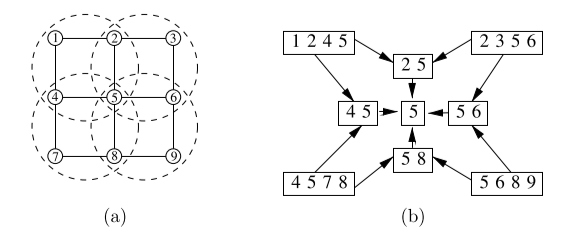
\includegraphics[width=.9\linewidth]{figure/4-5.PNG}
    \caption{
        (a) 叠加在 $3 \times 3$ 网格图上的 Kikuchi 簇。
        (b) 由 Kikuchi 簇给出的超图。
    }\label{fig:4-5}
\end{figure}

\subsection{广义信念传播}

原则上来说,变分问题 (4.53) 可以通过很多方法进行求解。
在这里我们描述一种基于 Lagrangian 的消息传递算法,这也是 Bethe 近似下的原始 Sum-product 算法的一种泛化。
这个方法的特点是消息只从父节点传递到子节点,也就是沿着超图的偏序集表示下的有向边传递。

在基于超树的变分问题 (4.53) 中,变量为每条超边 $h \in E$ 上的伪边际 $\tau_h$。
与前面对 Sum-product 算法的推导一样,这个优化问题的 Lagrangian 形式可以导出基于消息传递机制表示下的伪边际,其中的消息与 Lagrange 乘子有关。
原始问题有多种 Lagrangian 形式,从而可以导出多种消息传递算法。
在这里我们给出由 Yedidia et al. 推导的 Parent-to-child 形式的消息传递算法。

为了描述消息传递的更新机制,我们对给定的超边 $h$ 定义如下形式的后代集合(Descendants)与祖先集合(Ancestors):
\begin{equation}
    \mathcal{D}(h) := \{g \in E| g \subset h\}, \quad \mathcal{A}(h) := \{g \in E| g \supset h\}.
\end{equation}
例如,对于图 \ref{fig:4-4}(c) 中的超边 $h = (1245)$,我们有 $\mathcal{A}(h) = \emptyset, \mathcal{D}(h) = \{(25), (45), (5)\}$。
此外,我们定义 $\mathcal{D}^+(h) := \mathcal{D}(h) \cup \{h\}$ 以及 $\mathcal{A}^+(h) := \mathcal{A}(h) \cup \{h\}$。

给定一对超边 $(f, g)$,令 $M_{f \rightarrow g}(x_g)$ 代表从超边 $f$ 传递到超边 $g$ 的“消息”。
具体说来,这个消息是 $x_g$ 的状态空间上的一个函数(在离散情况下是一个多维数组)。
伪边际 $\tau_h$ 在这种 Parent-to-child 消息传递机制下的表示为:
\begin{equation}
    \tau_h(x_h) \propto \left[\prod_{g \in \mathcal{D}^+(h)}\psi_g(x_g; \theta)\right]\left[\prod_{g \in \mathcal{D}^+(h)}\prod_{f \in Par(g)/\mathcal{D}^+(h)}M_{f \rightarrow g}(x_g)\right], 
\end{equation}
式中 $\psi_g(x_g; \theta) = \exp(\theta(x_g))$。
伪边际 $\tau_h$ 的计算中包含了集合 $\mathcal{D}^+(h)$ 内每条超边 $g$ 的一个可计算函数 $\psi_g$。
此外,伪边际 $\tau_h$ 还需要从每条超边 $f \in Par(g)/\mathcal{D}^+(h)$ 中收集消息。
接下来我们通过对例 4.6 继续进行讨论来说明这种构造。

\begin{tcolorbox}
\begin{exam}[Kikuchi 近似下的 Parent-to-child 消息传递]

我们依旧采用图 \ref{fig:4-5} 中的 $3 \times 3$ 格点的 Kikuchi 近似来举例理解 Parent-to-child 消息传递机制。
首先考虑超边 $(1245)$,式 (4.56) 中的第一项是 $\mathcal{D}^+(1245)$ 中元素 $g$ 的可计算函数 $\psi_g$ 的乘积,本例中为 $\psi_{1245}\psi_{25}\psi_{45}\psi_5$。
然后考虑 $\mathcal{D}^+(1245)$ 中元素的父节点超边(但不包括 $\mathcal{D}^+(1245)$ 内部已有的超边)的消息的乘积。
图 \ref{fig:4-6}(a) 给出了相关示意,集合 $\mathcal{D}^+\{(1245)\}$ 由虚线椭圆中的超边给出。
在本例中,集合 $\bigcup_gPar(g)/\mathcal{D}^+(h)$ 为 $\{(2356), (4578)\}$,也就是 $(25), (45)$ 与 $(56), (58)$ 分别组合的父节点,这些超边也都是超边 $(5)$ 的父节点。
整体的结果如下:
\begin{align*}
    \tau_{1245} \propto &\psi_{12}'\psi_{14}'\psi_{25}'\psi_{45}'\psi_1'\psi_2'\psi_4'\psi_5' \\
    &\times M_{(2356)\rightarrow(25)}M_{(4578)\rightarrow(45)}M_{(56)\rightarrow 5}M_{(58)\rightarrow 5}.
\end{align*}
由于对称性,其他四个超边上的伪边际的表达式是类似的。
$\tau_{45}$ 和 $\tau_5$ 的表达式也可以通过类似的论证给出:
\begin{align*}
    \tau_{45} &\propto \psi_{45}'\psi_4'\psi_5'M_{(1245)\rightarrow(45)}M_{(4578)\rightarrow(45)}M_{(25)\rightarrow 5}M_{(56)\rightarrow 5}M_{(58)\rightarrow 5} \\
    \tau_5 &\propto \psi_5'M_{(45)\rightarrow 5}M_{(25)\rightarrow 5}M_{(56)\rightarrow 5}M_{(58)\rightarrow 5}.
\end{align*}

\end{exam}
\end{tcolorbox}

\begin{figure}[htbp]
    \centering
    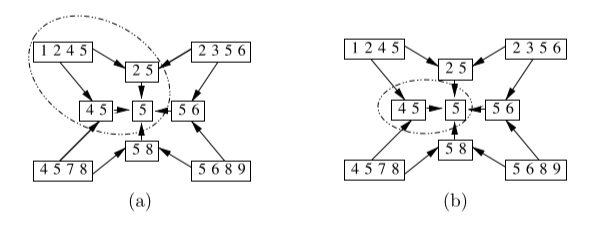
\includegraphics[width=.9\linewidth]{figure/4-6.PNG}
    \caption{
        Kikuchi 近似下的 Parent-to-child 消息传递机制示意。
        (a) 超边 $(1245)$ 的消息传递。
        后代集合 $\mathcal{D}^+\{(1245)\}$ 采用虚线椭圆框起来了。
        与 $\tau_{1245}$ 有关的父节点 包括集合 $\{(2356), (4578), (56), (58)\}$。
        (b) 超边 $(45)$ 的消息传递。
        后代集合 $\mathcal{D}^+\{(45)\}$ 同样采用虚线椭圆框起来了。
        相关的父节点集合为 $\{(1245), (4578), (25), (56), (58)\}$。
    }\label{fig:4-6}
\end{figure}

一般形式的 Sum-product 消息传递通过消息更新来保证 $\mathcal{L}(G)$ 中元素的边际化约束。
命题 4.2 的证明过程给出了消息更新的不动点满足 Lagrangian 公式的必要平稳条件。
关于一般化的 Sum-product 变体的细节可以在其他的论文中找到。

\section{期望传播算法}

在 Sum-product 算法的激励下,许多其他的消息传递算法也得到了发展。
例如 Minka 的 Expectation-propagation 算法族,相关的一类假定密度滤波方法(Assumed Density Filtering Methods),Expectation-consistent 推断,结构化 Summary-propagation 算法,以及 Opper 与 Winther 的自适应 TAP 方法。
这些算法通常是根据局部局匹配(Moment-matching)更新序列来定义的,是基于变分原理的个体更新,而不是整体逼近。
在本节中,我们将这些算法归纳到变分推理的框架之下,也就是证明它们是命题 3.4 中精确变分原理的特殊近似。

最早的假定密度滤波是在时间序列应用中发展起来的,最基本的模型就是图 \ref{fig:2-4} 所示的隐马尔可夫模型(HMM)。
我们之前已经讨论过,离散变量下的 HMM 的边际分布可以使用 Forward-backward 算法进行计算,这也是 Sum-product 算法的一个实例。
相似地,对于 Gauss-Markov 过程,Kalman 滤波可以计算 HMM 每个节点的均值与方差。
然而,对于一般化的连续变量隐马尔可夫模型而言,从节点 $t$ 传递给 $s$ 的消息 $M_{ts}$ 是一个实值函数,因此很难表示\footnote{
    Gaussian 情况是特例,因为它的消息函数总可以用均值和方差进行参数化表达,这也是 Kalman 滤波有效的基础。
}。假定密度滤波(ADF)的目的是为了绕过消息函数相关的计算困难,因此采用了消息函数的近似形式来进行操作,亦即利用某些合适的可计算类函数来对消息函数进行近似。
例如一般的连续消息可以近似为 Gaussian 消息。
如果采用 Kullback-Leibler 散度来度量接近度,那么计算消息近似的过程就能用 Moment-matching 操作来进行表示。

Minka 观察到 ADF 的基本思想可以不局限于马尔可夫链进而推广到任意图模型,这一见解构成了 Expectation-propagation(EP)算法族的基础。
与 ADF 一样,EP 及其相关算法通常利用 Moment-matching 操作来描述。
到目前为止,这些算法与 Bethe 近似之间的密切联系似乎并没有得到广泛的重视。
在本节中,我们将证明这些算法是求解命题 3.4 中精确变分原理的某些使用 Bethe-like 近似熵以及集合 $\mathcal{M}$ 上特定的凸外边界的松弛方法。
更具体地说,我们将证明 EP 的 Moment-matching 更新实际是求解优化问题的 Lagrangian 方法的一种特例,从而表明 EP 算法与 Belief-propagation 算法属于同一类变分方法。

\subsection{基于解耦项的近似熵}

我们首先基于对一个比较棘手的项式集合进行解耦的操作来给出一类一般的近似熵。
对给定的随机变量集合 $(X_1, \cdots, X_m) \in \mathbb{R}^m$,考虑将充分统计量进行如下分组:
\begin{equation}
    \underbrace{\phi := (\phi_1, \cdots, \phi_{d_T}),}_{\text{Tractable component}} \quad \underbrace{\Phi := (\Phi^1, \Phi^2, \cdots, \Phi^{d_I}),}_{\text{Intractable component.}}
\end{equation}
式中 $\phi_i$ 为单元统计量而 $\Phi^i$ 一般为多元统计量。
在下面的例子中我们会清楚地看到这个分组可以将相关的指数族分布的可处理分量与难处理分量分开。

我们需要为 $(\phi, \Phi)$ 的一些子集构建相关的指数族。
首先考虑容易处理的分量,向量值函数 $\phi: \mathcal{X}^m \rightarrow \mathbb{R}^{d_T}$ 具有对应的正则参数向量 $\theta \in \mathbb{R}^{d_T}$。
然后考虑难以处理的分量,对于每个 $i = 1, \cdots, d_I$,函数 $\Phi^i$ 将 $\mathcal{X}^m$ 映射到 $\mathbb{R}^b$,向量 $\tilde{\theta^i} \in \mathbb{R}^b$ 为相应的正则参数集。
总而言之,函数 $\Phi = (\Phi^1, \cdots, \Phi^{d_I})$ 将 $\mathcal{X}^m$ 映射到 $\mathbb{R}^{b\times d_I}$,相关的正则参数向量为 $\tilde{\theta} \in \mathbb{R}^{b\times d_I}$,可以被分组为 $\tilde{\theta} = (\tilde{\theta^1}, \tilde{\theta^2}, \cdots, \tilde{\theta^{d_I}})$。
这些充分统计量定义了如下指数族:
\begin{align}
    p(x; \theta, \tilde{\theta}) &\propto f_0(x)\exp(\langle\theta, \phi(x)\rangle)\exp(\langle\tilde{\theta}, \Phi(x)\rangle) \nonumber \\
    &= f_0(x)\exp(\langle\theta, \phi(x)\rangle)\prod_{i = 1}^{d_I}\exp(\langle\tilde{\theta^i}, \Phi^i(x)\rangle).
\end{align}
我们称任意具备 (4.58) 形式的密度 $p$ 属于 $(\phi, \Phi)$ 指数族。

接下来,我们定义如下基模型(Base Model):
\begin{equation}
    p(x; \theta, \vec{0}) \propto f_0(x)\exp(\langle\theta, \phi(x)\rangle), 
\end{equation}
在 $\tilde{\theta} = \vec{0}$ 的条件下难以处理的充分统计量 $\Phi$ 不起作用。
我们称任意具备 (4.59) 形式的分布 $p$ 属于 $\phi$ 指数族。
同样,对于任意 $i \in \{1, \cdots, d_I\}$,我们定义 $\Phi^i$ 增广分布(Augmented Distribution):
\begin{equation}
    p(x; \theta, \tilde{\theta^i}) \propto f_0(x)\exp(\langle\theta, \phi(x)\rangle)\exp(\langle\tilde{\theta^i}, \Phi^i(x)\rangle), 
\end{equation}
其中只引入了单项 $\Phi^i$,我们称任意具备 (4.60) 形式的分布 $p$ 属于 $(\phi, \Phi^i)$ 指数族。

对 $\phi, \Phi$ 进行 Tractable-Intractable 分组的基本前提是:
\begin{itemize}
    \item 第一,对于满足基本型 (4.59) 的分布(也就是 $\phi$ 指数族的成员)来说可以在多项式时间内精确计算出边际。
    \item 第二,对于任意 $i = 1, \cdots, d_I$,同样可以在多项式时间内精确计算满足基本型 (4.60) 的分布(也就是 $(\phi, \Phi^i)$ 指数族)的边际。
    \item 第三,对于全 $(\phi, \Phi)$ 指数族 (4.58) 而言很难执行精确计算,因为需要考虑所有项 $(\Phi^1, \Phi^2, \cdots, \Phi^{d_I})$。
\end{itemize}

\begin{tcolorbox}
\begin{exam}[混合模型的 Tractable-Intractable 分组]

我们以 Gaussian 混合模型为例来理解 (4.58) 的分配模式。
假设随机向量 $X \in \mathbb{R}^m$ 具有多元 Gaussian 分布,$N(0, \Sigma)$。
令 $\varphi(y; \mu, \Lambda)$ 表示分布为 $N(\mu, \Lambda)$ 的随机向量的密度,考虑以下两个成分的 GMM
\begin{equation}
    p(y| X = x) = (1-\alpha)\varphi(y; 0, \sigma_0^2I) + \alpha\varphi(y; x, \sigma_1^2I), 
\end{equation}
其中 $\alpha \in (0, 1)$ 代表混合权重,$\sigma_0^2$ 和 $\sigma_1^2$ 为方差,$I$ 为 $m \times m$ 的单位矩阵。

给定采样自混合密度 (4.61) 的 $n$ 个 i.i.d. 样本 $(y^1, y^2, \cdots, y^n)$,我们需要计算 $X$ 的后验分布的边际。
假设 $X$ 满足多元 Gaussian 先验 $X \sim N(0, \Sigma)$,使用 Bayes 定理可得后验形式为:
\begin{align}
    p(x|y^1, \cdots, y^n) &\propto \exp(-\frac{1}{2}x^T\Sigma^{-1}x)\prod_{i = 1}^np(y^i|X = x) \nonumber \\
    &= \exp(-\frac{1}{2}x^T\Sigma^{-1}x)\exp\left\{\sum_{i = 1}^n\log p(y^i|X = x)\right\}.
\end{align}

将这个模型转化为分组指数族 (4.58) 的形式,我们首先注意到 $\exp(-\frac{1}{2}x^T\Sigma^{-1}x)$ 能够用基本型 $f_0(x)\exp(\langle\theta, \phi(x)\rangle)$ 进行表示,因此有 $d_T = m$。
另一方面,我们对 $i = 1, \cdots, n$ 定义 $\Phi^i(x) := \log p(y^i|X = x)$。
应当指出的是这种定义是合理的,因为 $y^i$ 实际上是定值。
由以上定义可知 $\exp\{\sum_{i = 1}^n\log p(y^i|X = x)\}$ 实际就是式 (4.58) 中的乘积 $\prod_{i = 1}^{d_I}\exp(\langle\tilde{\theta^i}, \Phi^i(x)\rangle)$。
注意此处 $d_I = n, b = 1$,对于 $i = 1, \cdots, n$ 有 $\tilde{\theta^i} = 1$。

作为 $(\phi, \Phi)$ 指数族的一个例子,基础分布 $p(x; \theta, \vec{0}) \propto \exp(-\frac{1}{2}x^T\Sigma^{-1}x)$ 是一个多元 Gaussian,其边际可以在 $\mathcal{O}(m^3)$ 内精确计算出来。
同样地,对于 $i = 1, \cdots, n$,由 $\Phi^i$ 参数化表达的分布 (4.60) 与下式成正比:
\begin{equation}
    \exp(-\frac{1}{2}x^T\Sigma^{-1}x)[(1-\alpha)\varphi(y^i; 0, \sigma_0^2I)+\alpha\varphi(y^i; x, \sigma_1^2I)].
\end{equation}
这是一个具有两个成分的混合 Gaussian,因此也可以在立方时间内对边际进行精确计算。
然而,全分布 (4.62) 是一个具有 $2^n$ 个成分的混合 Gaussian,因此对边际进行精确计算的时间复杂度是问题规模的指数级。

\end{exam}
\end{tcolorbox}

回到主线,我们继续探索式 (4.58) 的一些性质。
作为一个指数族,其同样具有均值参数 $(\mu, \tilde{\mu}) \in \mathbb{R}^{d_T}\times\mathbb{R}^{d_I\times b}$,其中
\begin{equation*}
    \mu = \mathbb{E}[\phi(X)], \quad (\tilde{\mu}^1, \cdots, \tilde{\mu}^{d_I}) = \mathbb{E}[\Phi^1(X), \cdots, \Phi^{d_I}(X)].
\end{equation*}
作为一个指数族,命题 3.4 给出的一般变分原理同样适用。
变分原理 (3.45) 中的均值参数集合为
\begin{equation}
    \mathcal{M}(\phi, \Phi) := \{(\mu, \tilde{\mu})|(\mu, \tilde{\mu}) = \mathbb{E}_p[(\phi(X), \Phi(X))] \text{ for some } p\}, 
\end{equation}
熵(也就是负对偶函数)$H(\mu, \tilde{\mu}) = -A^*(\mu, \tilde{\mu})$。
我们的假设是,在全分布 (4.58) 下无法进行精确计算,因此均值空间 (4.64) 与熵函数的计算一定也存在相应的困难。
因此,我们现在根据分布的划分结构 (4.58) 来描述这些量的自然近似,从而得到一类 Expectation-propagation 算法。

与基分布 (4.59) 相关的均值参数集合为
\begin{equation}
    \mathcal{\phi} := \{\mu \in \mathbb{R}^{d_T}|\mu = \mathbb{E}_p[\phi(X)] \text{ for some density } p\}, 
\end{equation}
因此基分布也可以看做是一个 $d_T$ 维度的指数族。
根据命题 3.3,对于任意 $\mu \in \mathcal{M}^\circ(\phi)$,总是可以由一个指数族成员 $p_{\theta(\mu)}$ 导出。
此外,我们假设基分布容易计算,因此其熵函数 $H(\mu)$ 是可以直接得到的。
同样地,对于每一个 $i = 1, \cdots, d_I$,$\Phi^i$ 增广分布 (4.60) 也具有其均值参数空间 $\mathcal{M}(\phi, \Phi^i)$
\begin{equation}
    \{(\mu, \tilde{\mu}^i) \in \mathbb{R}^{d_T}\times\mathbb{R}^b| (\mu, \tilde{\mu}^i) = \mathbb{E}_p[(\phi(X), \Phi^i(X))] \text{ for some density } p\}.
\end{equation}
同理,对于任意 $(\mu, \tilde{\mu}^i) \in \mathcal{M}^\circ(\phi, \Phi^i)$,也都有一个 $(\phi, \Phi^i)$ 指数族成员可以得到这样的均值参数。
此外,因为 $\Phi^i$ 增广分布 (4.60) 容易计算,均值参数集合 $\mathcal{M}(\phi, \Phi^i)$ 以及熵函数 $H(\mu, \tilde{\mu}^i)$ 也是可以直接得到的。

有了这些基本概念,我们现在可以为集合 $\mathcal{M}(\phi, \Phi)$ 定义一个外边界。
给定某个均值参数候选集 $(\tau, \tilde{\tau}) \in \mathbb{R}^{d_T}\times\mathbb{R}^{d_I\times b}$,对任意 $i = 1, 2, \cdots, d_I$ 我们都定义一个坐标投影算子 $\Pi^i : \mathbb{R}^{d_T}\times\mathbb{R}^{d_I\times b} \rightarrow \mathbb{R}^{d_T}\times\mathbb{R}^b$:
\begin{equation*}
    (\tau, \tilde{\tau}) \xrightarrow{\Pi^i} (\tau, \tilde{\tau}^i) \in \mathbb{R}^{d_T}\times\mathbb{R}^b.
\end{equation*}
我们再定义集合
\begin{equation}
    \mathcal{L}(\phi; \Phi) := \{(\tau, \tilde{\tau})| \tau \in \mathcal{M}(\phi), \Pi^i(\tau, \tilde{\tau}) \in \mathcal{M}(\phi, \Phi^i) \forall i = 1, \cdots, d_I\}.
\end{equation}
注意有 $\mathcal{L}(\phi, \Phi)$ 为一个凸集,并且它也是原均值参数集合 $\mathcal{M}(\phi; \Phi)$ 的一个外边界。

我们现在给出熵函数的近似来适配结构 $\mathcal{L}(\phi; \Phi)$。
首先对于任意 $(\tau, \tilde{\tau}) \in \mathcal{L}(\phi, \Phi)$ 以及任意的 $i = 1, \cdots, d_I$,都有一个均值参数为 $(\tau, \tilde{\tau}^i)$ 的 $(\phi, \Phi^i)$ 指数族与之对应。
令 $H(\tau, \tilde{\tau}^i)$ 表示该指数族成员的熵。
同样地,根据 $\mathcal{L}(\phi; \Phi)$ 的定义有 $\tau \in \mathcal{M}(\phi)$,因此也存在一个均值参数为 $\tau$ 的 $\phi$ 指数族;我们将它的熵表示为 $H(\tau)$。
有了以上概念,我们定义如下的 Term-by-term 近似熵:
\begin{equation}
    H_{ep}(\tau, \tilde{\tau}) := H(\tau) + \sum_{l = 1}^{d_I}[H(\tau, \tilde{\tau}^l) - H(\tau)].
\end{equation}
结合近似熵与凸边界 (4.67) 可得优化问题
\begin{equation}
    \max_{(\tau, \tilde{\tau}) \in \mathcal{L}(\phi; \Phi)}\{\langle\tau, \theta\rangle + \langle\tilde{\tau}, \tilde{\theta}\rangle + H_{ep}(\tau, \tilde{\tau})\}.
\end{equation}
该优化问题即为命题 3.4 给出的精确变分原理的针对 $(\phi, \Phi)$ 指数族 (4.58) 的近似版本,这也是 Expectation-propagation 算法的基础。
如下面的例子所示,该优化问题与 Bethe 变分原理也关系密切。

\begin{tcolorbox}
\begin{exam}[Sum-product 与 Bethe 近似]

为了便于理解,我们现在从变分原理 (4.69) 的角度来考虑 Bethe 近似。
更具体地说,我们将从 Term-by-term 近似熵 (4.68) 中导出 Bethe 近似熵 (4.14),同时从 $\mathcal{M}(\phi, \Phi)$ 的凸外界 (4.67) 中导出式 (4.7) 中的基于树的外边界 $\mathcal{L}(G)$。

考虑一个基于无向图 $G = (V, E)$ 的成对 MRF,其每个节点 $s \in V$ 对应的变量离散为 $X_s \in \{0, 1, \cdots, r_s-1\}$;
和我们先前所看到的一样,它也可以借助指示函数和标准过完备参数化 (3.34) 表示为如 (4.1) 形式的指数族。
采用式 (4.69) 的观点,我们将充分统计量进行如下划分。
与节点相关的充分统计量定义为可处理集,与连边相关的统计量定义为难处理集。
借助式 (4.2) 中定义的函数 $\theta_s$ 和 $\theta_{st}$,基分布 (4.59) 可以表示为
\begin{equation}
    p(x; \theta_1, \cdots, \theta_m, \vec{0}) \propto \prod_{s \in V}\exp(\theta_s(x_s)).
\end{equation}
在这个例子中,$\Phi^i$ 项与函数 $\theta_{st}$ 相关联,也就是索引 $i$ 取值自图的连边集合。
对于每条边 $(u, v)$,$\Phi^{uv}$ 增广分布 (4.60) 具有以下形式:
\begin{equation}
    p(x; \theta_1, \cdots, \theta_m, \theta_{uv}) \propto [\prod_{s \in V}\exp(\theta_s(x_s))]\exp(\theta_{us}(x_u, x_v)).
\end{equation}

标准过完备表示的均值参数为 Singleton 和 Pairwise 的边际分布,我们使用 $(\tau_s, s \in V)$ 与 $\tau_{uv}$ 分别进行表示。
基分布的熵只取决于 Singleton 的边际,借助 (4.70) 的乘积结构,其简单形式为
\begin{equation*}
    H(\tau_1, \cdots, \tau_m) = \sum_{s \in V}H(\tau_s), 
\end{equation*}
其中 $H(\tau_s) = -\sum_{x_s}\tau_s(x_s)\log\tau_s(x_s)$ 就是边际分布的熵。
同样地,由于增广分布 (4.71) 只在无环图上添加并分解了一条边,其熵具有显式形式
\begin{align*}
    H(\tau_1, \cdots, \tau_m, \tau_{uv}) &= \sum_{s \in V}H(\tau_s) + [H(\tau_{uv}) - H(\tau_u) - H(\tau_v)] \\
    &= \sum_{s \in V}H(\tau_s) - I(\tau_{uv}), 
\end{align*}
其中 $H(\tau_{uv}) := -\sum_{x_u, x_v}\tau_{uv}(x_u, x_v)\log\tau_{uv}(x_u, x_v)$ 为联合熵,$I(\tau_{uv}) := H(\tau_u) + H(\tau_v) - H(\tau_{uv})$ 为互信息。
将这些碎片结合在一起,我们可以发现 Term-by-term 近似熵 (4.68) 在这个特定的问题下的形式为:
\begin{equation*}
    H_{ep}(\tau) = \sum_{s \in V}H(\tau_s) - \sum_{(s, t) \in E}I_{st}(\tau_{st}), 
\end{equation*}
这也就是式 (4.14) 所定义的 Bethe 近似熵。

接下来,我们将展示由式 (4.67) 定义的外边界 $\mathcal{L}(\phi; \Phi)$ 是如何导出 $\mathbb{L}(G)$ 的。
考虑局部候选边际分布集合
\begin{equation*}
    \tau = (\tau_s, s \in V; \tau_{st}, (s, t) \in E).
\end{equation*}
在现有的设定里,集合 $\mathcal{M}(\phi)$ 对应于分解分布下所有可实现边际 $(\tau_s, s \in V)$ 的集合,因此包含关系 $(\tau_s, s \in V) \in \mathcal{M}(\phi)$ 与非负性约束 $\forall s \in V: \tau_s(x_s) \geq 0$ 以及局部归一化约束
\begin{equation}
    \forall s \in V: \sum_{x_s}\tau_s(x_s) = 1
\end{equation}
等价。
注意到索引 $i$ 取值于图的连边集合;以 $i = (u, v)$ 为例,投影边际 $\Pi^{uv}(\tau)$ 为 $(\tau_1, \cdots, \tau_m, \tau_{uv})$。
集合 $\mathcal{M}(\phi; \Phi^{uv})$ 为所有这种形式的全局一致边际,并且与边际多面体 $\mathbb{M}(G_{uv})$ 等价,其中 $G_{uv}$ 表示仅有一条边 $(u, v)$ 的图。
由于这个图是树结构的,因此包含关系 $\Pi^{uv}(\tau) \in \mathcal{M}(\phi; \Phi^{uv})$ 与让 $\Pi^{uv}(\tau)$ 满足非负性约束以及局部归一化约束 (4.72) 条件,也就是边际化条件
\begin{equation*}
    \sum_{x_v}\tau_{uv}(x_u, x_v) = \tau_u(x_u), \quad \sum_{x_u}\tau_{uv}(x_u, x_v) = \tau_v(x_v)
\end{equation*}
等价。
因此,当 $(u, v)$ 取遍图的连边集合 $E$ 上时,包含关系 $\Pi^{uv}(\tau) \in \mathcal{M}(\phi; \Phi^{uv})$ 的全集给出了与式 (4.7) 定义的一阶松弛约束集合 $\mathbb{L}(G)$ 相同的条件。

\end{exam}
\end{tcolorbox}

\subsection{矩匹配的最优性}

回到主线上,我们现在推导解决 Expectation-propagation 变分原理 (4.69) 的 Lagrangian 方法。
我们将会展示这些 Lagrangian 更新实际上就是 Moment-matching,因此也包含了一般的 Expectation-propagation 更新。

我们基于以下两个基本步骤进行 Lagrangian 形式化:
\begin{itemize}
    \item 首先,我们扩大要进行优化的伪均值参数空间,使得定义 $\mathcal{L}(\phi; \Phi)$ 的原始约束解耦。
    \item 然后,我们用 Lagrange 乘子作为罚项引入新的约束,以使得最后的约束就是 $\mathcal{L}(\phi; \Phi)$ 中的成员所需要的。
\end{itemize}
首先开始增广步骤,我们将向量 $\tau \in \mathbb{R}^{d_T}$ 复制 $d_I$ 次,得到 $d_I$ 个新的向量 $\eta^i \in \mathbb{R}^{d_T}$ 并引入新的约束 $\forall i = 1, \cdots, d_I: \eta^i = \tau$。
由此可得到伪均值参数集合
\begin{equation*}
    \{\tau, (\eta^i, \tilde{\tau}^i), i = 1, \cdots, d_I\} \in \mathbb{R}^{d_T}\times(\mathbb{d_T}\times\mathbb{R}^b)^{d_I}, 
\end{equation*}
然后我们利用这些伪均值参数重新组织变分原理 (4.69):
\begin{equation}
    \max_{\{\tau, (\eta^i, \tilde{\tau}^i)\}}\left\{\langle\tau, \theta\rangle + \sum_{i = 1}^{d_I}\langle\tilde{\tau}^i, \tilde{\theta}^i\rangle + \underbrace{H(\tau) + \sum_{i = 1}^{d_I}[H(\eta^i, \tilde{\tau}^i) - H(\eta^i)]}_{F(\tau; (\eta^i, \tilde{\tau}^i))} \right\}, 
\end{equation}
其约束为 $\forall i = 1, \cdots, d_I: (\eta^i, \tilde{\tau}^i) \in \mathcal{M}(\phi; \Phi^i)$ 以及
\begin{equation}
    \tau = \eta^i \quad \forall i = 1, \cdots, d_I.
\end{equation}

现在让我们考虑一个特殊的迭代方案来解决问题 (4.73)。
特别地,对于每一个 $i = 1, \cdots, d_I$,定义一个与约束 $\tau = \eta_i$ 相关联的 Lagrange 乘子向量 $\lambda^i \in \mathbb{R}^{d_T}$。
我们可以得到 Lagrangian 函数
\begin{equation}
    L(\tau; \lambda) = \langle\tau, \theta\rangle + \sum_{i = 1}^{d_I}\langle\tilde{\tau}^i, \tilde{\theta}^i\rangle + F(\tau; (\eta^i, \tilde{\tau}^i)) + \sum_{i = 1}^{d_I}\langle\lambda^i, \tau-\eta^i\rangle.
\end{equation}
这个 Lagrangian 只是一部分,因为我们强迫满足约束 $\tau \in \mathcal{\phi}$ 以及 $(\eta^i, \tilde{\tau}^i) \in \mathcal{M}(\phi; \Phi^i)$。

考虑优化问题 (4.73) 的一个最优解 $\{\tau, (\eta^i, \tilde{\tau}^i), i = 1, \cdots, d_I\}$,这个解满足:
(a) 向量 $\tau$ 属于相对内点集 $\mathcal{M}^\circ(\phi)$,
(b) 对于每个 $i = 1, \cdots, d_I$,向量 $(\eta^i, \tilde{\tau}^i)$ 属于相对内点集 $\mathcal{M}^\circ(\phi; \Phi^i)$。
任何解都必须满足部分 Lagrangian (4.75) 相关的零梯度条件,也就是
\begin{subequations}
\begin{align}
    \nabla_{\tau}L(\tau; \lambda) &= 0, \\
    \nabla_{(\eta^i, \tilde{\tau}^i)}L(\tau; \lambda) &= 0 \quad \text{for } i = 1, \cdots, d_I, \\
    \nabla_{\lambda}L(\tau; \lambda) &= 0.
\end{align}
\end{subequations}

由于向量 $\tau$ 属于 $\mathcal{M}^\circ(\phi)$,因此它给定了 $\phi$ 指数族中的一个分布。
通过计算 Lagrangian 条件 (4.76a) 并进行简单的代数运算,我们发现这个指数族分布可以采用原始的参数向量 $\theta$ 以及 Lagrange 乘子 $\lambda$ 写为如下形式:
\begin{equation}
    q(x; \theta, \lambda) \propto f_0(x)\exp\left\{\langle\theta+\sum_{i = 1}^{d_I}\lambda^i, \phi(x)\rangle\right\}.
\end{equation}

同样地,对于每个 $i = 1, \cdots, d_I$,向量 $(\tau, \tilde{\tau}^i)$ 属于 $\mathcal{M}^\circ(\phi; \Phi^i)$,它也给定了 $(\phi, \Phi^i)$ 指数族中的一个分布。
对条件 (4.76b) 进行计算可知该分布可以表示为
\begin{equation}
    q^i(x; \theta, \tilde{\theta}^i, \lambda) \propto f_0(x)\exp(\langle\theta+\sum_{l \neq i}\lambda^l, \phi(x)\rangle + \langle\tilde{\theta}^i, \Phi^i(x)\rangle).
\end{equation}

最后的 Lagrangian 条件 (4.76c) 保证约束 (4.74) 得到满足。
注意到 $\tau = \mathbb{E}_q[\phi(X)]$ 以及 $\eta^i = \mathbb{E}_{q^i}[\phi(X)]$,这些约束可以得到 Moment-matching 条件
\begin{equation}
    \int q(x; \theta, \lambda)\phi(x)\nu(dx) = \int q^i(x; \theta, \tilde{\theta}^i, \lambda)\phi(x)\nu(dx), 
\end{equation}
对于 $i = 1, \cdots, d_I$ 成立。

基于式 (4.77),(4.78) 以及 (4.79),我们得到了 Expectation-propagation 更新,总结如图 \ref{fig:4-7} 所示。
可以看到算法的定义是合理的,因为对于任何可实现的均值参数 $\tau$,式 (4.81) 总会有一个解 $\lambda^{i(n)}$。
通过考虑由 $(\lambda^{i(n)}, \phi)$ 所定义的 $d_T$ 维度指数族,然后应用命题 3.3 就可以得到这个事实。
此外,这些 EP 更新的任何不动点都满足 (4.73) 优化所给出的 Lagrangian 条件。
基于这一点,我们提出一个重要结论,也就是假设优化问题 (4.73) 最少有一个最优点,那么 EP 更新的不动点一定存在。
与 Sum-product 算法与 Bethe 变分原理一样,EP 更新在一般情况下不能保证收敛。
然而,开发至少能找到变分问题 (4.73) 或等价的 (4.69) 的局部最优解的收敛算法相对简单,沿着为普通 Bethe 变分问题或其凸型版本开发的收敛算法的思路或许就能得到。

\begin{figure}[htbp]
    \textbf{Expectation-propagation (EP) 更新:}
    
    (1) 在 $n = 0$ 次迭代时,初始化 Lagrange 乘子向量 $(\lambda^1, \cdots, \lambda^{d_I})$。 
    
    (2) 在 $n = 1, 2, \cdots$ 的每次迭代中选择某个索引 $i(n) \in \{1, \cdots, d_I\}$,然后
        
    \quad (a) 使用式 (4.78) 构建增广分布 $q^{i(n)}$ 并且计算均值参数
        \begin{equation}
            \eta^{i(n)} := \int q^{i(n)}(x)\phi(x)\nu(dx) = \mathbb{E}_{q^{i(n)}}[\phi(X)].
        \end{equation}
    
    \quad (b) 使用式 (4.77) 构建基分布 $q$ 并且调整 $\lambda^{i(n)}$ 以满足 Moment-matching 条件
        \begin{equation}
            \mathbb{E}_q[\phi(X)] = \eta^{i(n)}.
        \end{equation}
    \caption{
        Expectation-propagation 更新的相关步骤。
        这是解决类 Bethe 问题 (4.73) 或等价的 (4.69) 的一种 Lagrangian 算法。
    }\label{fig:4-7}
\end{figure}

从更高的角度来看,一些关键要素如下:
在变分框架中,Expectation-propagation 算法是基于类 Bethe 的近似熵 (4.68) 以及均值参数集合的一个特定凸外界 (4.67)。
此外,EP 算法中的 Moment-matching 步骤来自于尝试解决变分原理 (4.69) 的一种 Lagrangian 方法。

最后,我们举例说明图 \ref{fig:4-7} 中算法的具体形式:

\begin{tcolorbox}
\begin{exam}[作为 Moment-matching 的 Sum-product]
    作为例 4.9 的后续,我们现在展示图 \ref{fig:4-7} 中的更新式 (4.80) 与 (4.81) 得到 Sum-product 更新的过程。
    在这个例子中,索引 $i$ 取值于图的连边集合。
    与 $i = (u, v)$ 相关的 Lagrange 乘子为 $(\lambda_{uv}(x_v), \lambda_{vu}(x_u))$。
    基分布 (4.77) 采用这些量可以写为
    \begin{align}
        q(x; \theta, \lambda) &\propto \prod_{s \in V}\exp(\theta_s(x_s))\prod_{(u, v) \in E}\exp(\lambda_{uv}(x_v)+\lambda_{vu}(x_u)) \nonumber \\
        &= \prod_{s \in V}\exp(\theta_s(x_s) + \sum_{t \in N(s)}\lambda_{ts}(x_s)), 
    \end{align}
    或者更简洁点,$q(x; \theta, \lambda) \propto \prod_{s \in V}\tau_s(x_s)$,其中我们定义伪边际
    \begin{equation*}
        \tau_s(x_s) \propto \exp(\theta_s(x_s)+\sum_{t \in N(s)}\lambda_{ts}(x_s)).
    \end{equation*}
    值得注意的是 Singleton 伪边际 $\tau_s$ 与由命题 4.2 得到的 Sum-product 表达式 (4.23) 之间的相似性。
    同样,当 $l = (u, v)$,增广分布 (4.78) 可以写为
    \begin{align}
        q^{(u, v)}(x; \theta, \lambda) &\propto q(x; \theta, \lambda)\exp(\theta_{uv}(x_u, x_v) - \lambda_{vu}(x_u) - \lambda_{uv}(x_v)) \nonumber \\
        &= [\prod_{s \in V}\tau_s(x_s)]\exp(\theta_{uv}(x_u, x_v)-\lambda_{vu}(x_u)-\lambda_{uv}(x_v)).
    \end{align}

    现在考虑更新式 (4.80) 与 (4.81)。
    如果 $i = (u, v)$,那么更新式 (4.80) 与计算分布 (4.83) 的 Singleton 边际等价。
    更新式 (4.81) 规定 Lagrange 乘子 $\lambda_{uv}(x_v)$ 与 $\lambda_{vu}(x_u)$ 必须得到调整以使得分布 (4.82) 的边际 $\{\tau_u, \tau_v\}$ 和这些边际相匹配。
    通过一些代数运算,这些不动点条件可以得到在边 $(u, v)$ 上的 Sum-product 更新,其中的消息是由指数化的 Lagrange 乘子给出的 $M_{uv}(x_v) = \exp(\lambda_{uv}(x_v))$。
\end{exam}
\end{tcolorbox}

从 Term-by-term 的观点来看,Sum-product 算法使用了基分布的乘积(参见式 (4.70))。
一个很自然的拓展是考虑具有更多结构的基分布。

\begin{tcolorbox}
\begin{exam}[树结构的 EP]
    我们将通过导出树结构的 EP 算法来解释这个想法,并将其应用在具有图结构 $G = (V, E)$ 的成对 MRF 上。
    我们使用与例 4.9 以及 例 4.10 相同的设定和参数化形式。
    给定这个图的某个生成树 $T = (V, E(T))$,基分布 (4.59) 为
    \begin{equation}
        p(x; \theta, \vec{0}) \propto \prod_{s \in V}\exp(\theta_s(x_s))\prod_{(s, t) \in E(T)}\exp(\theta_{st}(x_s, x_t)).
    \end{equation}
    在这个例子中,索引 $i$ 取值 $(u, v) \in E/E(T)$;
    给定边 $(u, v)$,$\Phi^{uv}$ 增广分布 (4.60) 可以通过添加项 $\theta_{uv}$ 得到:
    \begin{equation}
        p(x; \theta, \theta_{uv}) \propto p(x; \theta, \vec{0})\exp(\theta_{uv}(x_u, x_v)).
    \end{equation}

    我们现在描述集合 $\mathcal{M}(\phi, \Phi)$,$\mathcal{M}(\phi)$ 以及 $\mathcal{M}(\phi, \Phi^i)$ 在这种设定下的类比。
    首先,如例 4.9 所示,与全模型 (4.58) 相应的均值参数子向量为
    \begin{equation*}
        \mu := (\mu_s, s \in V; \mu_{st}, (s, t) \in E).
    \end{equation*}
    据此,$\mathcal{M}(\phi, \Phi)$ 的类比就是边际多面体 $\mathbb{M}(G)$。
    其次,如果我们使用树结构分布 (4.84) 作为基分布,相关均值参数的子向量为
    \begin{equation*}
        \mu(T) := (\mu_s, s \in V; \mu_{st}, (s, t) \in E(T)).
    \end{equation*}
    集合 $\mathcal{M}(\phi)$ 的类比就是边际多面体 $\mathbb{M}(T)$,或者等价的 —— 根据命题 4.1 —— 为集合 $\mathbb{L}(T)$。
    最后,如果我们使用边 $i = (u, v) \notin E(T)$,那么集合 $\mathcal{M}(\phi, \Phi^i)$ 的类比就是边际多面体 $\mathbb{M}(T \cup (u, v))$。

    集合 $\mathcal{L}(\phi; \Phi)$ 的类比比较有趣,我们将其称为边际多面体 $\mathbb{M}(G)$ 的 tree-EP 外界。
    它包含向量 $\tau = (\tau_s, s \in V; \tau_{st}, (s, t) \in E)$,这些向量满足
    \begin{itemize}
        \item[(a)] 包含关系 $\tau(T) \in \mathbb{M}(T)$ 成立,
        \item[(b)] 对于所有 $(u, v) \notin T$,包含关系 $(\tau(T), \tau_{uv}) \in \mathbb{M}(T \cup (u, v))$ 成立。
    \end{itemize}
    可以看到这么定义的集合含于 $\mathbb{L}(G)$:特别地,条件 $\tau(T) \in \mathbb{M}(T)$ 保证了与树结构相应的所有边际分布的非负性,归一性以及边际性,并且包含关系 $(\tau(T), \tau_{uv}) \in \mathbb{M}(T \cup (u, v))$ 保证了 $\tau_{uv}$ 是非负的,同时也满足与 $\tau_u$ 与 $\tau_v$ 之间的边际化关系。
    对于带环图,tree-EP 外边界严格含于 $\mathbb{L}(G)$;例如,当应用于三节点的单环 $C_3$ 上时,tree-EP 外边界和边际多面体等价。
    但是如例 4.1 所示,集合 $\mathbb{M}(C_3)$ 严格含于 $\mathbb{L}(C_3)$。
    
    tree-EP 相应的近似熵 $H_{ep}$ 很容易定义。
    给定在 tree-EP 外边界中的伪均值参数 $\tau$ 的候选集合,我们定义与基分布 (4.84) 相关的树结构熵
    \begin{equation}
        H(\tau(T)) := \sum_{s \in V}H(\tau_s) - \sum_{(s, t) \in E(T)}I_{st}(\tau_{st}).
    \end{equation}
    同样,对于每条边 $(u, v) \notin E(T)$,我们定义与增广分布 (4.85) 相对应的熵 $H(\tau(T), \tau_{uv})$;
    与基分布不同,这个熵没有精确形式(因为图不是联合树形式),但是它也很容易计算。
    tree-EP 近似熵的形式如下:
    \begin{equation*}
        H_{ep}(\tau) = H(\tau(T)) + \sum_{(u, v) \notin E(T)}[H(\tau(T), \tau_{uv}) - H(\tau(T))].
    \end{equation*}

    最后,我们导出 tree-EP 的 Moment-matching 更新式 (4.80) 与 (4.81)。
    对于每条边 $(u, v) \notin E(T)$,令 $\lambda^{uv}(T)$ 表示 Lagrange 乘子向量,与 $\tau(T)$ 的维度相同,再令 $\phi(x; T)$ 表示与 $T$ 相关的充分统计量的子集。
    优化后的基分布 (4.77) 可以使用原始基分布 (4.84) 和这些 Lagrange 乘子重新写为
    \begin{equation*}
        q(x; \theta, \lambda) \propto p(x; \theta, \vec{0})\prod_{(u, v) \notin E(T)}\exp(\langle\lambda^{uv}(T), \phi(x; T)\rangle).
    \end{equation*}
    如果边 $(u, v)$ 被加进去,增广分布 (4.78) 可以重新写为
    \begin{equation*}
        q^{uv}(x; \theta, \lambda) \propto p(x; \theta, \vec{0})\exp(\theta_{uv}(x_u, x_v))\prod_{(s, t) \neq (u, v)}\exp(\langle\lambda^{uv}(T), \phi(x; T)\rangle).
    \end{equation*}
    对于一个给定的边 $(u, v) \notin E(T)$,Moment-matching 步骤 (4.81) 与在分布 $q^{uv}(x; \theta, \lambda)$ 下为连边 $(s, t) \in E(T)$ 计算 Singleton 边际与 Pairwise 边际有关。
    步骤 (4.81) 与更新 Lagrange 乘子 $\lambda^{uv}(T)$ 以使得对于所有节点 $s \in V$ 以及连边 $(s, t) \in E(T)$ 而言 $q(x; \theta, \lambda)$ 所给出的边际与 $q^{uv}(x; \theta, \lambda)$ 所给出的相一致。
\end{exam}
\end{tcolorbox}

之前的例子都只考虑了离散随机变量;我们现在转向考虑首次出现在例 4.8 中的带有连续变量的混合模型。

\begin{tcolorbox}
\begin{exam}[Gaussian 混合模型的 EP]
    重新回忆指数族形式的混合模型表达式 (4.62),其包括基础的势函数 $\phi(x) = (x; xx^T)$ 以及对于 $i = 1, \cdots, n$ 的辅助项 $\Phi^i(x) = \log p(y^i|x)$。
    现在转向多种均值参数空间的类比,集合 $\mathcal{M}(\phi; \Phi)$ 是 $\mathbb{R}^m \times \mathcal{S}_+^m \times \mathbb{R}^n$ 的子集,相应的全局可实现均值参数空间被划分为
    \begin{equation*}
        (\mathbb{E}[X]; \mathbb{E}[XX^T]; \mathbb{E}[\log p(y^i|X)], i = 1, \cdots, n).
    \end{equation*}
    注意 $(y^1, y^2, \cdots, y^n)$ 为已观测量,因此在整个推导过程中保持不变。

    集合 $\mathcal{M}(\phi)$ 是 $\mathbb{R}^m\times\mathcal{S}_+^m$ 的一个子集,与例 3.7 给出的一个多元 Gaussian 的均值参数空间相关。
    对于 $i = 1, \cdots, n$,约束集合 $\mathcal{M}(\phi; \Phi^i)$ 是 $\mathbb{R}^m\times\mathcal{S}_+^m\times\mathbb{R}$ 的一个子集,与具有如下划分形式的所有全局可实现的均值参数集合相关
    \begin{equation*}
        (\mathbb{E}[X], \mathbb{E}[XX^T], \mathbb{E}[\log p(y^i|X)]).
    \end{equation*}

    现在转向考虑多种熵函数,基本项是多元 Gaussian 的熵 $H(\mu)$,其中 $\mu$ 表示 $(\mathbb{E}[X], \mathbb{E}(XX^T))$;
    相似地,增广项 $H(\mu, \tilde{\mu}^i)$ 是具有充分统计量 $(\phi(x), \log p(y^i|x))$ 的指数族成员的熵,均值参数为 $(\mu, \tilde{\mu}^i)$,其中 $\tilde{\mu}^i = \mathbb{E}[\log p(y^i|X)]$。
    我们可以使用这些量定义变分原理 (4.69) 的一个类比。

    现在转向考虑 Moment-matching 步骤 (4.80) 与 (4.81),Gaussian-mixture EP 算法的 Lagrangian 形式可以采用 $n$ 个矩阵-向量 Lagrange 乘子对来构建
    \begin{equation*}
        (\lambda^i, \Lambda^i) \in \mathbb{R}^m \times \mathbb{R}^{m \times m}, i = 1, \cdots, n,
    \end{equation*}
    每一个都对应一个增广分布。
    由于 $X \sim N(0, \Sigma)$,优化基分布 (4.77) 可以采用 $\Sigma^{-1}$ 与 Lagrange 乘子写为
    \begin{equation}
        q(x; \Sigma; (\lambda, \Lambda)) \propto \exp\left\{\langle\sum_{i = 1}^n\lambda^i, x\rangle+\langle\langle-\frac{1}{2}\Sigma^{-1}+\sum_{i = 1}^n\Lambda^i, xx^T\rangle\rangle\right\}.
    \end{equation}
    值得指出的是,这是一个简单的多元 Gaussian 分布。
    对于任意 $i \in \{1, 2, \cdots, d_I\}$ 相应的增广分布 (4.78) $q^i$ 形式如下:
    \begin{equation}
        f_0(x)\exp\{\langle\sum_{l \neq i}\lambda^l, x\rangle+\langle\langle-\frac{1}{2}\Sigma^{-1}+\sum_{l \neq i}\Lambda^l, xx^T\rangle\rangle+\langle\tilde{\theta}_i, \log p(y^i|x)\rangle\}.
    \end{equation}
    有了这些条件,步骤 (4.80) 就与在分布 (4.88) 下计算均值参数 $(\mathbb{E}_{q^i}[X], \mathbb{E}_{q^i}[XX^T])$ 相关,步骤 (4.81) 就与调整多元 Gaussian (4.87) 以使其具有这些均值参数相关。
    这些 Moment-matching 更新的不动点满足对精确变分原理的类 Bethe 近似进行最优求解的必要的 Lagrangian 条件。

    我们推荐读者进一步阅读 Minka 与 Seeger 的相关工作,以了解更多有关 Gaussian-mixture EP 算法及其性质的细节。
\end{exam}
\end{tcolorbox}